\documentclass[11pt,a4paper,oneside]{report}

% ---------------------------------------------------------------------------
% Preamble
% ---------------------------------------------------------------------------
\usepackage[a4paper,margin=2.5cm,headheight=14pt,footskip=1.1cm]{geometry}
\usepackage{fancyhdr}
\usepackage{titlesec}
\usepackage{microtype}
\usepackage{lmodern}
\usepackage{booktabs}
\usepackage{array}
\usepackage{tabularx}
\usepackage{longtable}
\usepackage{graphicx}
\usepackage{caption}
\usepackage{subcaption}
\usepackage{xcolor}
\usepackage{amsmath,amssymb}
\usepackage{enumitem}
\usepackage[most]{tcolorbox}
\usepackage{listings}
\usepackage{tikz}
\usetikzlibrary{arrows.meta,positioning,shapes.geometric,fit,backgrounds,shadows}
\usepackage{needspace}
\usepackage[colorlinks=true,linkcolor=honestblue,citecolor=goodgreen,urlcolor=honestblue,linktoc=all,bookmarksnumbered=true]{hyperref}
\usepackage[capitalize,noabbrev]{cleveref}

% --- palette -----------------------------------------------------------------
% Matches lxnet/report.py:LIGHT exactly, so the report and the repository's
% own generated figures read as one visual system.
\definecolor{honestblue}{HTML}{2A78D6}
\definecolor{leakyorange}{HTML}{EB6834}
\definecolor{goodgreen}{HTML}{1BAF7A}
\definecolor{amberwarn}{HTML}{EDA100}
\definecolor{inkblack}{HTML}{0B0B0B}
\definecolor{mutedgray}{HTML}{52514E}
\definecolor{panelbg}{HTML}{F7F7F5}
\definecolor{rulegray}{HTML}{D8D7D0}

% --- chapter / section typography --------------------------------------------
\titleformat{\chapter}[display]
  {\normalfont\bfseries}
  {\filright\Large\color{mutedgray}\MakeUppercase{\chaptertitlename}\ \thechapter}
  {6pt}
  {\Huge\color{inkblack}}
  [{\vspace{8pt}\color{honestblue}\rule{\textwidth}{1.4pt}\vspace{4pt}}]
\titlespacing*{\chapter}{0pt}{0pt}{28pt}

\titleformat{\section}
  {\normalfont\Large\bfseries\color{inkblack}}{\thesection}{0.6em}{}
\titleformat{\subsection}
  {\normalfont\large\bfseries\color{inkblack}}{\thesubsection}{0.6em}{}
\titleformat{\subsubsection}
  {\normalfont\normalsize\bfseries\color{mutedgray}}{\thesubsubsection}{0.6em}{}

% --- headers / footers --------------------------------------------------------
\pagestyle{fancy}
\fancyhf{}
\fancyhead[L]{\small\color{mutedgray}\nouppercase{\leftmark}}
\fancyhead[R]{\small\color{mutedgray}\nouppercase{\rightmark}}
\renewcommand{\headrulewidth}{0.6pt}
\renewcommand{\headrule}{\color{rulegray}\hrule height\headrulewidth width\headwidth}
\fancyfoot[L]{\small\color{mutedgray}LXNet Technical Report}
\fancyfoot[R]{\small\color{mutedgray}\thepage}
\renewcommand{\footrulewidth}{0pt}
\fancypagestyle{plain}{%
  \fancyhf{}
  \fancyfoot[L]{\small\color{mutedgray}LXNet Technical Report}
  \fancyfoot[R]{\small\color{mutedgray}\thepage}
  \renewcommand{\headrulewidth}{0pt}
}
\renewcommand{\chaptermark}[1]{\markboth{#1}{}}
\renewcommand{\sectionmark}[1]{\markright{#1}}

% --- callout boxes -------------------------------------------------------------
\newtcolorbox{warningbox}[1][]{%
  colback=leakyorange!7, colframe=leakyorange!65!black,
  title=Not a Medical Device, fonttitle=\bfseries,
  coltitle=white, colbacktitle=leakyorange!80!black,
  boxrule=0.8pt, arc=1.5pt, left=6pt, right=6pt, top=3pt, bottom=3pt, #1}
\newtcolorbox{notebox}[2][]{%
  colback=honestblue!5, colframe=honestblue!55!black,
  title=#2, fonttitle=\bfseries,
  coltitle=white, colbacktitle=honestblue!65!black,
  boxrule=0.8pt, arc=1.5pt, left=6pt, right=6pt, top=3pt, bottom=3pt, #1}
\newtcolorbox{debtbox}[1][]{%
  colback=amberwarn!10, colframe=amberwarn!70!black,
  title=Documented Engineering Debt, fonttitle=\bfseries,
  coltitle=inkblack, colbacktitle=amberwarn!55,
  boxrule=0.8pt, arc=1.5pt, left=6pt, right=6pt, top=3pt, bottom=3pt, #1}

% --- code listings ---------------------------------------------------------
\lstdefinestyle{pystyle}{
  language=Python,
  basicstyle=\ttfamily\small,
  keywordstyle=\color{honestblue}\bfseries,
  commentstyle=\color{mutedgray}\itshape,
  stringstyle=\color{goodgreen!60!black},
  numbers=left,
  numberstyle=\tiny\color{mutedgray},
  numbersep=8pt,
  frame=single,
  rulecolor=\color{rulegray},
  framesep=5pt,
  breaklines=true,
  breakatwhitespace=false,
  showstringspaces=false,
  tabsize=4,
  captionpos=b,
  backgroundcolor=\color{panelbg},
  xleftmargin=1em,
  xrightmargin=0.4em,
}
\lstset{style=pystyle}
\renewcommand{\lstlistingname}{Listing}
\renewcommand{\bibname}{References}

% --- misc ---------------------------------------------------------------------
\setlength{\parskip}{2pt}
\emergencystretch=3em
\setlist[itemize]{topsep=3pt,itemsep=2pt}
\setlist[enumerate]{topsep=3pt,itemsep=2pt}
\graphicspath{{../}}
\newcommand{\LXNet}{\textsc{LXNet}}
\newcommand{\code}[1]{\texttt{\small #1}}

\title{LXNet Technical Report}
\author{baveshraam}
\date{August 2026}

% ===========================================================================
\begin{document}
\pagenumbering{roman}

% ---------------------------------------------------------------------------
% Title page
% ---------------------------------------------------------------------------
\begin{titlepage}

\begin{tikzpicture}[remember picture,overlay]
  \draw[honestblue,line width=2.6pt]
    ([xshift=2.5cm,yshift=-2.7cm]current page.north west) --
    ([xshift=-2.5cm,yshift=-2.7cm]current page.north east);
  \draw[rulegray,line width=1.2pt]
    ([xshift=2.5cm,yshift=2.7cm]current page.south west) --
    ([xshift=-2.5cm,yshift=2.7cm]current page.south east);
\end{tikzpicture}
\vspace*{1.6cm}
{\small\color{mutedgray}\MakeUppercase{Technical Report}\hfill\MakeUppercase{Version 1.0}}\\[2.2cm]
{\fontsize{46}{50}\selectfont\bfseries LXNet}\\[0.35cm]
{\Large\color{mutedgray} Engineering an Honest Evaluation for a\\[2pt] Lightweight Chest Radiograph Classifier}\\[1.4cm]
{\large A replication study of Humayan~et~al.\ (PLOS~One, 2026), instrumented to
measure and remove near-duplicate leakage in a nine-class chest X-ray corpus,
with a full account of the data, training, evaluation and interpretability
engineering behind the result.}
\vfill
\begin{tcolorbox}[colback=panelbg,colframe=rulegray,boxrule=0.6pt,arc=1pt,
  left=10pt,right=10pt,top=8pt,bottom=8pt,width=\textwidth]
\small
\begin{tabularx}{\linewidth}{@{}l X@{}}
\textbf{Author} & baveshraam \\
\textbf{Repository} & \url{https://github.com/baveshraam/LXNet} \\
\textbf{Subject system} & \LXNet{} v1.0.0 --- 356{,}585-parameter CNN, 9-class chest radiograph classifier \\
\textbf{Reference work} & Humayan et al., \textit{A Lightweight CNN for Lung Disease
Classification from Chest X-ray with XAI-based Interpretability}, PLOS One, 2026 \\
\textbf{Status} & Measured results current as of the \texttt{runs/grouped} and
\texttt{runs/random} training arms, seed 42 \\
\textbf{Scope} & Research artefact. Not validated for, and not to be used in,
clinical decision-making. \\
\end{tabularx}
\end{tcolorbox}
\vspace{0.4cm}
\end{titlepage}

% ---------------------------------------------------------------------------
% Abstract
% ---------------------------------------------------------------------------
\chapter*{Abstract}
\addcontentsline{toc}{chapter}{Abstract}
The dataset underlying this system contains the same chest radiograph saved
repeatedly under different filenames: 6{,}657 byte-unique image files reduce to
4{,}635 visually distinct X-rays once near-duplicate copies are collapsed by
perceptual hashing --- roughly 30\% of the corpus is redundant. A model
evaluated on a naive random split is scored, in part, on pictures it has
already seen during training. Under that protocol, \LXNet{} reaches 95.4\%
hold-out accuracy; once every re-saved copy of an X-ray is confined to a
single split, the same model, the same weights procedure, and the same
preprocessing score 92.9\%. The 2.5-point gap is not model skill --- it is
leakage, and it is measured directly in this report rather than assumed.

This document describes the complete system built to make that measurement,
and to make every other reported number in the repository trustworthy in the
same way: dataset indexing and deduplication, perceptual near-duplicate
grouping, group-aware stratified splitting and cross-validation, a cached
CLAHE preprocessing pipeline, the \LXNet{} architecture and three
transfer-learning baselines (DenseNet201, InceptionV3, ResNet50V2), the
training and early-stopping regime, the evaluation and significance-testing
methodology, three interpretability methods (Grad-CAM, Score-CAM, LIME), the
inference path, and the automated test suite that pins each of these
guarantees against regression. Measured results are reported for both the
honest (group-aware) and leaky (random) split protocols on identical data,
identical preprocessing and identical model code, so the cost of the leak can
be read off directly rather than inferred.

The headline engineering trade is explicit: \LXNet{} gives up 5.6 percentage
points of accuracy to the strongest baseline (ResNet50V2, 98.5\%) in exchange
for a 63$\times$ improvement in accuracy per parameter (260.5 vs.\ 4.1 per
million parameters). Which side of that trade is correct depends entirely on
the deployment target, and this report treats that as an engineering decision
rather than a foregone conclusion.

\begin{warningbox}
This system is a research artefact evaluated on one public dataset of
undocumented clinical provenance. Pneumonia recall is 73.2\%: roughly one in
four pneumonia films is missed. Nothing in this report should be read as
supporting diagnostic, triage, or screening use. See \cref{ch:limitations}.
\end{warningbox}

% ---------------------------------------------------------------------------
% Front matter
% ---------------------------------------------------------------------------
\clearpage
\tableofcontents
\clearpage
\listoffigures
\clearpage
\listoftables
\clearpage

\chapter*{Glossary of Abbreviations}
\addcontentsline{toc}{chapter}{Glossary of Abbreviations}
\begin{table}[h]
\centering
\small
\begin{tabular}{@{}ll@{}}
\toprule
\textbf{Term} & \textbf{Meaning} \\
\midrule
CAM & Class Activation Map \\
CLAHE & Contrast Limited Adaptive Histogram Equalisation \\
CV & Cross-Validation \\
dhash & Difference hash (perceptual image fingerprint) \\
F1 (macro) & Harmonic mean of precision and recall, unweighted across classes \\
GAP & Global Average Pooling \\
Grad-CAM & Gradient-weighted Class Activation Mapping \\
LIME & Local Interpretable Model-agnostic Explanations \\
LOC & Lines of code \\
pp & Percentage points \\
ReLU & Rectified Linear Unit \\
Score-CAM & Score-weighted Class Activation Mapping \\
TF & TensorFlow \\
XAI & Explainable Artificial Intelligence \\
\bottomrule
\end{tabular}
\caption{Abbreviations used throughout this report.}
\end{table}

\clearpage
\pagenumbering{arabic}

% ===========================================================================
\chapter{Introduction}
\label{ch:intro}

\section{Problem Statement}

Humayan et al.\ \cite{humayan2026} propose a 0.35-million-parameter
convolutional network for classifying chest radiographs into nine disease
categories, arguing that a model two orders of magnitude smaller than a
standard ImageNet backbone can match its accuracy. That is a strong,
falsifiable claim, and it depends entirely on the evaluation being clean: if
the test set contains images the model has already seen in some form during
training, the accuracy gap between a large and small model collapses for a
reason that has nothing to do with either architecture.

The dataset used in the replication --- \emph{X-Ray Lung Diseases Images (9
classes)} \cite{kaggle-dataset} --- turns out to have exactly that problem.
Chest radiographs are collected, re-exported, and re-uploaded across medical
imaging repositories, and this corpus is no exception: the same film appears
multiple times under different filenames, at different JPEG quality, in
different color modes. \Cref{ch:dataset} quantifies this precisely. The
consequence for evaluation is direct --- a conventional random train/test
split does not guarantee that a test image is unseen, only that its
\emph{filename} was not used for training.

\section{What This System Does}

\LXNet{} is both a re-implementation of the architecture proposed in
\cite{humayan2026} and an evaluation harness built specifically to answer one
question honestly: \emph{once every near-duplicate copy of an X-ray is kept
on one side of the split, how much of the reported accuracy survives?} The
system:

\begin{enumerate}
\item indexes, hashes, and deduplicates the raw dataset (\cref{ch:dataset});
\item builds a perceptual near-duplicate graph and derives a
  \emph{group-aware} stratified split and $k$-fold cross-validation, so no
  evaluation image has a training-set twin (\cref{ch:dataset});
\item preprocesses every image once with CLAHE and caches the result, rather
  than repeating an expensive CPU-bound transform every epoch
  (\cref{ch:preprocessing});
\item trains \LXNet{} and three transfer-learning baselines --- DenseNet201,
  InceptionV3, ResNet50V2 --- under an identical protocol
  (\cref{ch:architecture,ch:training});
\item evaluates every model with macro-averaged metrics and a paired
  significance test across cross-validation folds (\cref{ch:evaluation});
\item explains individual predictions with Grad-CAM, Score-CAM and LIME
  (\cref{ch:xai});
\item exposes a validated, file-based inference path with an explicit trust
  boundary (\cref{ch:inference}); and
\item pins every one of the above guarantees with an automated test suite
  that runs in continuous integration (\cref{ch:testing}).
\end{enumerate}

\section{Why This Report Exists}

The repository's \texttt{README.md} and \texttt{docs/RESULTS.md} answer
\emph{what the numbers are}. This report answers \emph{why the system is
built the way it is} --- the internal data structures, the ordering
constraints between deduplication, splitting and balancing, the reasoning
behind each hyperparameter and architectural choice, and the specific
regression each test in the suite exists to catch. It is written for an
engineer who needs to modify, extend, or audit the system, not only read its
headline numbers.

\section{Document Roadmap}

\Cref{ch:architecture} gives the system-level view: module responsibilities,
their dependencies, and the two data flows (training and inference) that
thread through them. \Cref{ch:dataset,ch:preprocessing} cover the data layer
in depth --- indexing, deduplication, perceptual grouping, splitting, and the
cached preprocessing pipeline. \Cref{ch:architecture-model,ch:training,ch:evaluation}
cover the model, the training loop, and the metrics. \Cref{ch:results}
reports measured outcomes. \Cref{ch:xai,ch:inference} cover interpretability
and deployment. \Cref{ch:testing} maps the test suite to the guarantees it
protects. \Cref{ch:decisions} is a standalone ledger of the non-obvious
engineering trade-offs made throughout, with rationale. \Cref{ch:limitations}
states, without hedging, what this system does not know how to do.
\Cref{ch:reproducibility} gives the exact commands and seeds needed to
regenerate every number in this report.

% ===========================================================================
\chapter{System Architecture}
\label{ch:architecture}

\section{Package Layout}

The system is a single installable Python package, \code{lxnet}, exposing
four console entry points (\code{lxnet-train}, \code{lxnet-predict},
\code{lxnet-report}, \code{lxnet-explain}) over ten modules. There is no
service layer, no configuration-file system, and no plugin architecture ---
every module is imported directly by the module that needs it, and every
tunable parameter is a CLI flag or a function default. For a system with one
dataset, one architecture family, and one deployment target (a local
checkpoint file), this is a deliberate ceiling: an abstraction layer for
multiple datasets or model registries would be undirected complexity with no
second consumer to justify it.

\begin{table}[h]
\centering
\small
\begin{tabularx}{\linewidth}{@{}l X@{}}
\toprule
\textbf{Module} & \textbf{Responsibility} \\
\midrule
\code{data.py} & Dataset indexing, SHA-256 deduplication, perceptual
  (dhash) near-duplicate grouping, group-aware stratified splitting and
  $k$-fold cross-validation, class balancing. \\
\code{preprocess.py} & CLAHE contrast equalisation and single-image loading
  for inference. \\
\code{pipeline.py} & Bulk CLAHE preprocessing into a cached uint8 tensor;
  the \code{tf.data} pipeline that serves batches to training and evaluation. \\
\code{models.py} & The \LXNet{} architecture and the three
  transfer-learning baselines, behind one dispatch function. \\
\code{train.py} & CLI orchestration: hold-out training, $k$-fold
  cross-validation, the GPU guard, and \code{results.json} generation. \\
\code{evaluate.py} & Metric computation (macro precision/recall/F1,
  confusion matrix), per-fold summarisation, Wilcoxon signed-rank testing. \\
\code{xai.py} & Grad-CAM, Score-CAM and LIME implementations, plus heatmap
  overlay compositing. \\
\code{explain.py} & CLI driver that renders the per-class interpretability
  panel from a trained checkpoint. \\
\code{predict.py} & The inference trust boundary: input validation, the
  \code{Classifier} class, and the \code{lxnet-predict} CLI. \\
\code{report.py} & Turns \code{results.json} into every figure in
  \texttt{docs/} (light and dark themed) and the generated
  \texttt{docs/RESULTS.md}. \\
\bottomrule
\end{tabularx}
\caption{Module responsibilities. Ten modules, no layer of indirection
between a CLI flag and the function it configures.}
\label{tab:modules}
\end{table}

\section{Data Flow}

\Cref{fig:architecture} traces both flows through the system: the training
flow that produces a scored checkpoint, and the two consumers of that
checkpoint --- the interpretability panel and the inference CLI. Every arrow
in the diagram is a real function call or file artifact in the codebase; none
is aspirational.

\begin{figure}[htbp]
\centering
\resizebox{\textwidth}{!}{%
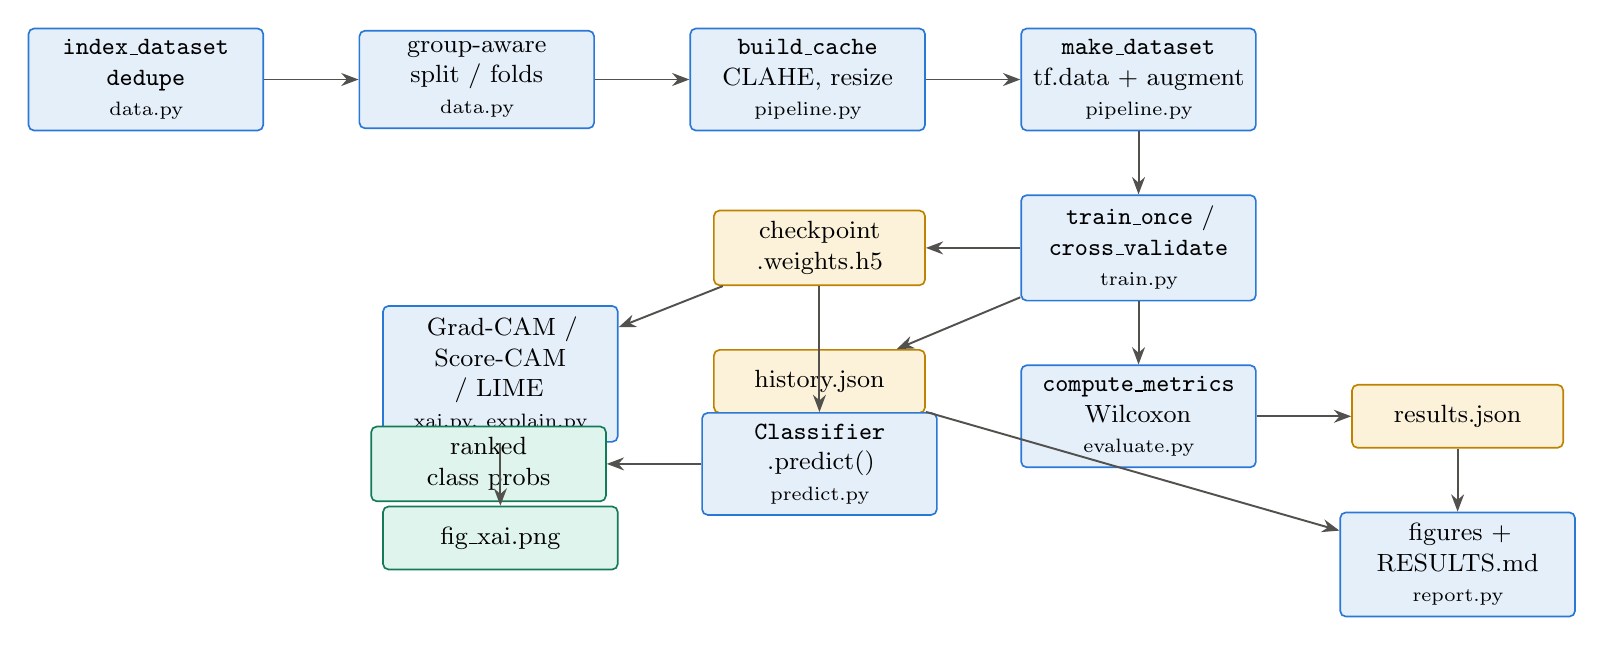
\begin{tikzpicture}[
  node distance=8mm and 12mm,
  every node/.style={font=\small},
  box/.style={draw=inkblack, rounded corners=2pt, fill=panelbg, minimum height=8mm,
              text width=27mm, align=center, inner sep=4pt, line width=0.6pt},
  proc/.style={box, fill=honestblue!12, draw=honestblue},
  art/.style={box, fill=amberwarn!15, draw=amberwarn!80!black, text width=24mm},
  term/.style={box, fill=goodgreen!14, draw=goodgreen!70!black},
  arr/.style={-{Stealth[length=2.2mm]}, line width=0.7pt, color=mutedgray},
]
  \node[proc] (index) {\code{index\_dataset}\\\code{dedupe}\\\scriptsize data.py};
  \node[proc, right=of index] (split) {group-aware\\split / folds\\\scriptsize data.py};
  \node[proc, right=of split] (cache) {\code{build\_cache}\\CLAHE, resize\\\scriptsize pipeline.py};
  \node[proc, right=of cache] (dataset) {\code{make\_dataset}\\tf.data + augment\\\scriptsize pipeline.py};
  \node[proc, below=of dataset] (train) {\code{train\_once} /\\\code{cross\_validate}\\\scriptsize train.py};
  \node[art, left=of train] (ckpt) {checkpoint\\.weights.h5};
  \node[art, below=of ckpt] (hist) {history.json};
  \node[proc, below=of train] (evaluate) {\code{compute\_metrics}\\Wilcoxon\\\scriptsize evaluate.py};
  \node[art, right=of evaluate] (results) {results.json};
  \node[proc, below=of results] (report) {figures +\\RESULTS.md\\\scriptsize report.py};
  \node[proc, left=of ckpt, yshift=-16mm] (explain) {Grad-CAM /\\Score-CAM / LIME\\\scriptsize xai.py, explain.py};
  \node[term, below=of explain] (xaifig) {fig\_xai.png};
  \node[proc, below=of ckpt, yshift=-8mm] (predict) {\code{Classifier}\\.predict()\\\scriptsize predict.py};
  \node[term, left=of predict] (predout) {ranked\\class probs};

  \draw[arr] (index) -- (split);
  \draw[arr] (split) -- (cache);
  \draw[arr] (cache) -- (dataset);
  \draw[arr] (dataset) -- (train);
  \draw[arr] (train) -- (ckpt);
  \draw[arr] (train) -- (hist);
  \draw[arr] (train) -- (evaluate);
  \draw[arr] (evaluate) -- (results);
  \draw[arr] (results) -- (report);
  \draw[arr] (hist) -- (report);
  \draw[arr] (ckpt) -- (explain);
  \draw[arr] (explain) -- (xaifig);
  \draw[arr] (ckpt) -- (predict);
  \draw[arr] (predict) -- (predout);
\end{tikzpicture}%
}
\caption{End-to-end data flow. Blue nodes are processing stages; amber nodes
are on-disk artifacts; green nodes are terminal outputs. The training flow
(top row into \code{train\_once}) produces a checkpoint that two independent
downstream consumers read: the interpretability panel and the inference
CLI. Neither consumer re-runs training or re-derives the split.}
\label{fig:architecture}
\end{figure}

\section{Two Independent Split Protocols, One Codebase}

A structural decision worth calling out on its own: \code{train.py} accepts
\code{-{}-split-mode \{grouped,random\}} and routes to either
\code{group\_aware\_split}/\code{group\_aware\_folds} or the naive
\code{stratified\_split} in \code{data.py}. The random path is not legacy
code kept for compatibility --- it is retained \emph{specifically} so the two
protocols can be run on identical images, identical preprocessing, and
identical model code, differing only in which split function partitions the
data. \Cref{ch:results} depends on this: the leakage measurement is only
meaningful because both arms share every other variable.

\section{Cross-Cutting Invariant: the Digest-to-Row Map}

Every module downstream of \code{pipeline.build\_cache} refers to images by
integer row index into a single cached tensor
(\texttt{runs/<name>/preprocessed.npz}), not by file path. \code{train.py}
maintains a \code{digest\_to\_row} dictionary (SHA-256 digest
$\rightarrow$ cache row) to translate between the \code{Sample} objects that
\code{data.py} works with --- which carry semantic identity (path, label,
digest) --- and the row indices that \code{pipeline.py} and \code{models.py}
consume. This indirection exists because splitting, grouping and folding are
naturally expressed over \code{Sample} objects, while the actual tensors fed
to Keras are naturally expressed as flat arrays. Any code that reintroduces a
positional assumption between the two (for instance, assuming cache row $i$
corresponds to \code{samples[i]} after a re-order) reintroduces the exact
image/label misalignment bug that \texttt{tests/test\_pipeline.py} exists to
catch (\cref{ch:testing}).

% ===========================================================================
\chapter{Dataset and Data Integrity}
\label{ch:dataset}

\section{Source Corpus}

The corpus is \emph{X-Ray Lung Diseases Images (9 classes)}
\cite{kaggle-dataset}: 6{,}743 image files under nine class directories, named
with a two-digit numeric prefix (\code{00}--\code{08}) followed by a
Portuguese class name. \code{data.py} sorts class directories by name and
assigns integer labels 0--8 by that sort order --- so the numeric prefix,
not the display label, is load-bearing; renaming a class directory without
preserving its prefix silently relabels every image in it.

\begin{table}[h]
\centering
\small
\begin{tabular}{@{}rlr@{\hspace{18pt}}rlr@{}}
\toprule
\textbf{Label} & \textbf{Class} & \textbf{Images} & \textbf{Label} & \textbf{Class} & \textbf{Images} \\
\midrule
0 & Normal & 1340 & 5 & Degenerative Infectious & 594 \\
1 & Pneumonia & 1060 & 6 & Encapsulated Lesions & 658 \\
2 & Higher Density & 678 & 7 & Mediastinal Changes & 596 \\
3 & Lower Density & 629 & 8 & Chest Changes & 544 \\
4 & Obstructive Pulmonary & 644 & & & \\
\bottomrule
\end{tabular}
\caption{Class distribution, 6{,}743 images total. Normal outnumbers Chest
Changes 2.5:1 --- macro-averaged metrics are used throughout
(\cref{ch:evaluation}) so this imbalance cannot hide in a headline number.}
\label{tab:class-dist}
\end{table}

An on-load audit (exercised by \texttt{tests/test\_data.py}) finds zero
corrupt files, 40 distinct image resolutions (6{,}263 of the 6{,}743 files are
$450\times450$), and a mix of grayscale, RGB and RGBA colour modes ---
consistent with images aggregated from more than one export pipeline rather
than one consistent acquisition system.

\section{Exact Deduplication}
\label{sec:exact-dedup}

Every file is hashed with SHA-256 on load (\code{data.\_digest}). Grouping by
digest finds 74 groups of byte-identical files, 84 excess copies in total,
and --- more seriously --- one image whose byte-identical copies are filed
under two contradictory classes (\emph{Pneumonia} and \emph{Lower Density}).
\code{data.dedupe} drops \emph{both} copies of a cross-class conflict rather
than picking one: keeping either would train the model on a coin flip for
that exact image, and there is no principled way to decide which label is
correct from the pixels alone.

\begin{lstlisting}[caption={Cross-class conflicts are dropped entirely, not
resolved by a heuristic (\texttt{lxnet/data.py}).}, label=lst:dedupe]
for group in by_digest.values():
    labels = {s.label for s in group}
    if len(labels) > 1:
        report.cross_class_conflicts += 1
        log.warning(
            "dropping %d copies of an image labelled as %s",
            len(group), sorted(s.class_name for s in group),
        )
        continue
    report.exact_duplicates += len(group) - 1
    kept.append(group[0])
\end{lstlisting}

Exact hashing only catches files that are bit-for-bit identical. It misses
the more common case on this dataset: the same X-ray, re-exported at a
different JPEG quality or resized, which flips most of the file's bytes while
leaving the image visually unchanged to a clinician --- and to a
convolutional network.

\section{Perceptual Near-Duplicate Grouping}
\label{sec:perceptual-grouping}

\subsection{Difference Hashing}

Visual identity is approximated with a \emph{difference hash} (dhash): each
image is converted to grayscale, downscaled to a $9\times8$ thumbnail, and
encoded as a 64-bit signature where bit $(i,j)$ is 1 if pixel $(i, j{+}1)$ is
brighter than pixel $(i, j)$. Downscaling to $9\times 8$ deliberately
discards resolution, compression artefacts and sensor noise, so a re-saved or
resized copy of the same film lands on the same, or a very close, digest.

\begin{lstlisting}[caption={The difference hash (\texttt{lxnet/data.py}).},
label=lst:dhash]
def _dhash(path_str: str, hash_size: int = 8) -> str:
    with Image.open(path_str) as im:
        thumb = im.convert("L").resize(
            (hash_size + 1, hash_size), Image.LANCZOS
        )
    a = np.asarray(thumb, dtype=np.int16)
    return np.packbits((a[:, 1:] > a[:, :-1]).flatten()).tobytes().hex()
\end{lstlisting}

\subsection{Why the Matching Threshold Is Exact, Not Fuzzy}

The natural extension --- treat two digests within a small Hamming distance
as the same image --- was measured and rejected. Chest radiographs are
near-identical \emph{by construction}: same anatomy, same framing convention,
low dynamic range. \Cref{tab:hamming} shows what happens to the largest
connected component as the tolerance is relaxed.

\begin{table}[h]
\centering
\small
\begin{tabular}{@{}lrrrr@{}}
\toprule
\textbf{Hamming threshold (bits)} & 0 & 1 & 2 & 3 \\
\midrule
Largest resulting group (images) & 21 & 143 & 374 & 1{,}680 \\
\bottomrule
\end{tabular}
\caption{Size of the largest perceptual-duplicate group as the matching
tolerance increases. At threshold 3 the largest group spans 8 of the 9
classes and has a median internal Hamming distance of 14 bits --- a
transitive-closure artefact of chaining near-matches, not a true duplicate
set.}
\label{tab:hamming}
\end{table}

At threshold 0 (exact digest equality), sampled matching pairs have a median
pixel correlation of 0.9913, against 0.4263 for random image pairs ---
strong evidence that an exact-digest match really is the same film re-saved,
and that the grouping does not need, and should not use, any tolerance at
all. \code{GROUP\_MAX\_DISTANCE = 0} in \code{data.py} encodes this
conclusion as a constant, with the measurement recorded alongside it in a
comment rather than left implicit.

\subsection{Union-Find Grouping}

Even at threshold 0, some images occupy more than one digest bucket after a
resize (a genuinely-tiny compression difference can flip a hash bit).
\code{group\_samples} therefore performs a full pairwise Hamming comparison
between all distinct digests, in $256\times N$ blocks to bound memory, and
unions any pair within \code{max\_distance} using a union-find structure:

\begin{lstlisting}[caption={Blocked pairwise Hamming distance plus union-find
(\texttt{lxnet/data.py}).}, label=lst:unionfind]
chunk = 256
for start in range(0, len(digests), chunk):
    block = bits[start : start + chunk]
    dist = _POPCOUNT[block[:, None, :] ^ bits[None, :, :]].sum(axis=2)
    for local_i, row in enumerate(dist):
        i = start + local_i
        for j in np.nonzero(row <= max_distance)[0]:
            if j > i:
                union(i, int(j))
\end{lstlisting}

With \code{max\_distance = 0} this loop is doing more work than strictly
necessary --- an exact-match grouping could be a single dictionary keyed by
digest --- but the general form is what makes the threshold in
\cref{tab:hamming} a one-line experiment rather than a rewrite, and the cost
is bounded ($O(N^2/256)$ comparisons over $N \approx 6{,}600$ digests,
each an 8-byte XOR-and-popcount) and pays for itself once at indexing time,
not once per training run.

\section{Group-Aware Splitting}
\label{sec:group-aware-split}

\Cref{fig:split-protocol} lays out the full pipeline from raw files to a
scored split, and the two protocols this system supports at the last step.

\begin{figure}[htbp]
\centering
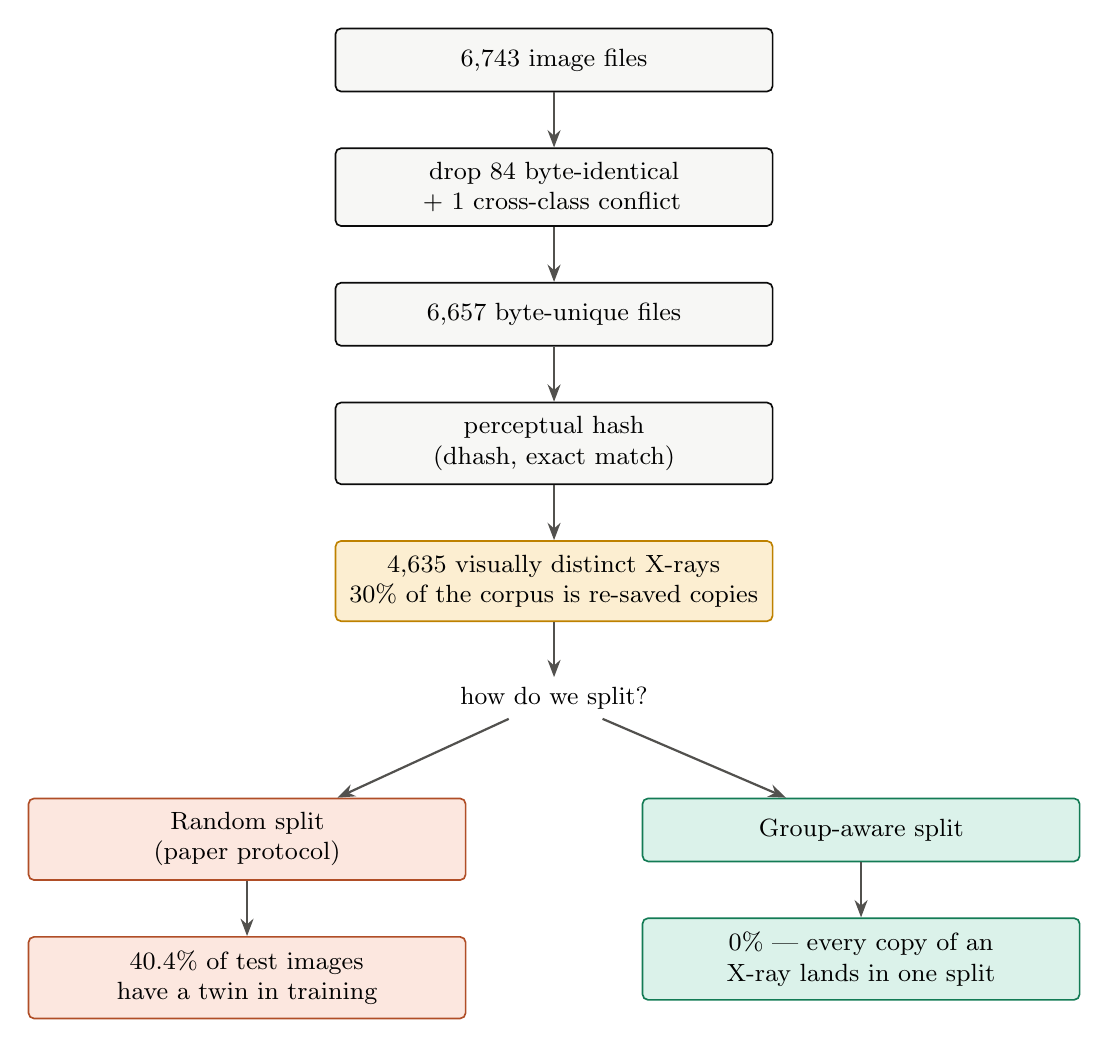
\begin{tikzpicture}[
  node distance=7mm and 7mm,
  every node/.style={font=\small, align=center},
  n/.style={draw=inkblack, rounded corners=2pt, fill=panelbg, minimum height=8mm,
            text width=52mm, inner sep=5pt, line width=0.6pt},
  hl/.style={n, fill=amberwarn!18, draw=amberwarn!80!black},
  bad/.style={n, fill=leakyorange!16, draw=leakyorange!75!black},
  good/.style={n, fill=goodgreen!16, draw=goodgreen!70!black},
  arr/.style={-{Stealth[length=2.2mm]}, line width=0.8pt, color=mutedgray},
]
  \node[n] (a) {6{,}743 image files};
  \node[n, below=of a] (b) {drop 84 byte-identical\\+ 1 cross-class conflict};
  \node[n, below=of b] (c) {6{,}657 byte-unique files};
  \node[n, below=of c] (d) {perceptual hash\\(dhash, exact match)};
  \node[hl, below=of d] (e) {4{,}635 visually distinct X-rays\\30\% of the corpus is re-saved copies};
  \node[below=of e, draw=none, fill=none] (f) {how do we split?};
  \node[bad, below left=10mm and -2mm of f] (g) {Random split\\(paper protocol)};
  \node[good, below right=10mm and -2mm of f] (h) {Group-aware split};
  \node[bad, below=of g] (i) {40.4\% of test images\\have a twin in training};
  \node[good, below=of h] (j) {0\% --- every copy of an\\X-ray lands in one split};

  \draw[arr] (a) -- (b);
  \draw[arr] (b) -- (c);
  \draw[arr] (c) -- (d);
  \draw[arr] (d) -- (e);
  \draw[arr] (e) -- (f);
  \draw[arr] (f) -- (g);
  \draw[arr] (f) -- (h);
  \draw[arr] (g) -- (i);
  \draw[arr] (h) -- (j);
\end{tikzpicture}
\caption{Both split protocols consume the identical 4{,}635-group corpus.
The only variable is whether a split boundary is allowed to cut through a
perceptual group.}
\label{fig:split-protocol}
\end{figure}

\code{stratified\_split} splits individual \emph{images}: it shuffles each
class's samples and slices by fraction, which guarantees per-class
proportions but says nothing about which images end up on which side of the
cut. \code{group\_aware\_split} instead treats each perceptual group as an
indivisible unit, assigns it the label its majority member carries, and deals
whole groups to train/val/test with a greedy quota rule: at each step, the
next group goes to whichever split is furthest below its target share of the
running total.

\begin{lstlisting}[caption={Greedy quota assignment keeps every split near its
target proportion while never splitting a group
(\texttt{lxnet/data.py:group\_aware\_split}).}, label=lst:groupsplit]
for idx in order:
    members = entries[idx]
    total = sum(counts.values()) + len(members)
    choice = max(targets, key=lambda k: targets[k] * total - counts[k])
    parts[choice].extend(members)
    counts[choice] += len(members)
\end{lstlisting}

$k$-fold cross-validation uses the same grouping through
\href{https://scikit-learn.org/stable/modules/generated/sklearn.model_selection.StratifiedGroupKFold.html}{\code{sklearn.model\_selection.StratifiedGroupKFold}}
\cite{pedregosa2011}, passing each sample's group id alongside its label so
every fold boundary is also group-clean.

\section{Balancing After Splitting, Not Before}
\label{sec:balance-order}

The reference paper balances classes before splitting. On a dataset with 30\%
redundancy, that ordering places duplicated copies of a minority-class image
on both sides of the eventual split --- oversampling manufactures the exact
leakage this system exists to remove, concentrated on the classes an
evaluator would trust least. \code{train.py} enforces the opposite order
unconditionally: split first, then oversample the training portion only.
\Cref{fig:pipeline-order} makes this explicit as an ordering constraint
rather than a convention.

\begin{table}[h]
\centering
\small
\begin{tabular}{@{}clp{7.2cm}@{}}
\toprule
\textbf{Step} & \textbf{Operation} & \textbf{Why this position in the sequence} \\
\midrule
1 & Index + SHA-256 hash & Establishes exact-duplicate identity before anything
  touches labels. \\
2 & Deduplicate & Removes byte-identical copies and cross-class conflicts;
  must precede perceptual grouping so groups are built on the reduced set. \\
3 & Perceptual grouping & Establishes which files are the same X-ray,
  independent of the eventual split. \\
4 & Group-aware split & Deals whole groups to train/val/test. Must precede
  balancing. \\
5 & Balance (oversample) & Applied to the \emph{training} split's rows only. \\
6 & Cache + train & The balanced, split-correct index is the only thing
  handed to \code{pipeline.build\_cache} for training. \\
\bottomrule
\end{tabular}
\caption{The load-bearing ordering. Swapping steps 4 and 5 reproduces the
leak this project exists to measure.}
\label{fig:pipeline-order}
\end{table}

Cross-validation applies the same discipline one level deeper: each fold's
early-stopping monitor is carved out of that fold's \emph{training} rows
before oversampling, so a duplicated minority-class row can never straddle
the monitor and the training set within a fold either. This is covered in
detail in \cref{sec:carve-validation}.

\section{Class Balancing Strategy}

Two balancing mechanisms exist in \code{data.py}: \code{oversample\_to\_balance},
which duplicates minority-class rows uniformly at random up to the majority
count, and \code{class\_weights}, which computes inverse-frequency sample
weights normalised to a mean of approximately 1. Only oversampling is wired
into the training CLI --- \code{train.py} calls
\code{\_oversample\_indices} on the training split and passes
\code{class\_weight=None} to \code{model.fit}. \code{class\_weights} is
correct, tested (\texttt{tests/test\_data.py}), and unused by default: it
remains available as a zero-duplication alternative for a future run that
wants to avoid inflating the training set's memory footprint, but changing
the default requires a deliberate decision, not a silent switch.

% ===========================================================================
\chapter{Preprocessing and the Input Pipeline}
\label{ch:preprocessing}

\section{CLAHE}

The reference paper's headline preprocessing step is Contrast Limited
Adaptive Histogram Equalisation. A chest radiograph carries its diagnostic
signal in a narrow band of greys, and global histogram equalisation over- or
under-corrects regions with very different local contrast (dense bone versus
soft lung parenchyma in the same frame). CLAHE addresses this by equalising
within local tiles and clipping the contrast amplification so that flat,
low-signal regions are not turned into noise.

\code{preprocess.apply\_clahe} wraps \code{cv2.createCLAHE} with a clip limit
of 2.0 and an $8\times 8$ tile grid (\cref{tab:clahe-params}), applied to a
single-channel grayscale image. Source files are collapsed to grayscale
\emph{before} CLAHE runs: applying CLAHE independently per RGB channel would
equalise each channel's contrast separately and shift the overall colour
balance, which is meaningless on a modality that carries no colour
information in the first place.

\begin{table}[h]
\centering
\small
\begin{tabularx}{\linewidth}{@{}ll X@{}}
\toprule
\textbf{Parameter} & \textbf{Value} & \textbf{Effect} \\
\midrule
\code{clipLimit} & 2.0 & Ceiling on local contrast amplification; higher
  values amplify sensor/compression noise in flat regions. \\
\code{tileGridSize} & $8\times 8$ & Number of local regions the image is
  independently equalised over. \\
Input & 2-D \code{uint8} & CLAHE is defined over a single intensity channel. \\
Output resolution & $224\times 224$ & Matches the input contract of all four
  model architectures (\cref{ch:architecture-model}). \\
\bottomrule
\end{tabularx}
\caption{CLAHE configuration, \texttt{lxnet/preprocess.py}.}
\label{tab:clahe-params}
\end{table}

After equalisation, images are resized to $224\times224$ with
\code{cv2.INTER\_AREA} (the appropriate interpolation kernel for
downsampling, as most source images exceed the target resolution), scaled to
$[0,1]$, and replicated across three channels. The channel replication is
what lets grayscale \LXNet{} and the ImageNet-pretrained RGB baselines
consume literally the same tensor --- a prerequisite for the parameter-count
comparison in \cref{ch:results} to be a fair one.

\section{Caching: Preprocess Once, Not Once per Epoch}
\label{sec:caching}

CLAHE runs on the CPU through OpenCV and is far too slow to repeat on every
training epoch. \code{pipeline.build\_cache} therefore decodes, CLAHE's and
resizes every sample exactly once, storing the result as an \code{(N, 224,
224)} \code{uint8} grayscale array at \texttt{runs/<name>/preprocessed.npz}.
\Cref{tab:cache-size} quantifies why the array is grayscale \code{uint8} and
not float32 RGB: channel replication and the $[0,1]$ cast happen inside the
\code{tf.data} graph, on the already-cached tensor, not before it is written
to disk.

\begin{table}[h]
\centering
\small
\begin{tabular}{@{}lrr@{}}
\toprule
\textbf{Representation} & \textbf{Bytes per image} & \textbf{Full corpus (6.7k images)} \\
\midrule
Grayscale \code{uint8}, cached & $224 \times 224 \times 1 = 50{,}176$ & $\approx$338\,MB \\
Float32 RGB, uncached & $224 \times 224 \times 3 \times 4 = 602{,}112$ & $\approx$4\,GB \\
\bottomrule
\end{tabular}
\caption{Storing the cache as grayscale \texttt{uint8} rather than
float32 RGB is a 12$\times$ reduction, entirely because channel replication
and float scaling are deferred to the \texttt{tf.data} graph.}
\label{tab:cache-size}
\end{table}

One implementation detail is load-bearing on Windows specifically:
\code{cv2.imread} cannot open a path containing non-ASCII characters, and the
source dataset's class directories are named in Portuguese. \code{build\_cache}
reads the file's bytes directly with \code{np.fromfile} and decodes them with
\code{cv2.imdecode}, sidestepping the OS path-handling layer entirely:

\begin{lstlisting}[caption={Reading by buffer, not by path, to survive
non-ASCII directory names (\texttt{lxnet/pipeline.py}).}, label=lst:imdecode]
buffer = np.fromfile(sample.path, dtype=np.uint8)
gray = cv2.imdecode(buffer, cv2.IMREAD_GRAYSCALE)
if gray is None:
    raise ValueError(f"could not decode image: {sample.path}")
\end{lstlisting}

If the cache file already exists, \code{build\_cache} loads it directly and
skips reprocessing; the file must be deleted manually to force a rebuild
after a preprocessing change (\cref{ch:decisions} discusses the trade-off
this implies).

\section{The \texttt{tf.data} Pipeline}

\code{pipeline.make\_dataset} wraps the cached array in a \code{tf.data}
pipeline that performs, in order: cast to \code{float32} and scale to
$[0,1]$, expand to a single channel dimension and replicate to three,
optional augmentation, batching, and prefetch with \code{AUTOTUNE}. Training
datasets are shuffled with a buffer of $\min(N, 4096)$ elements, reshuffled
every epoch; evaluation datasets are never shuffled, because downstream code
matches predictions to labels by array position, not by an explicit key.

\subsection{Augmentation Is Conservative by Clinical Reasoning, Not Just Convention}

\begin{lstlisting}[caption={The full augmentation policy
(\texttt{lxnet/pipeline.py}).}, label=lst:augment]
def _augment(x: tf.Tensor, seed: int) -> tf.Tensor:
    x = tf.image.random_flip_left_right(x)
    x = tf.image.random_brightness(x, max_delta=0.10)
    x = tf.image.random_contrast(x, lower=0.90, upper=1.10)
    return tf.clip_by_value(x, 0.0, 1.0)
\end{lstlisting}

Horizontal flip, and mild brightness/contrast jitter ($\pm10\%$ and
$0.90$--$1.10\times$ respectively) --- and nothing else. Vertical flip and
large-angle rotation are deliberately excluded: an upside-down chest
radiograph is not a plausible clinical acquisition, and left-right mirroring
is not always augmentation-neutral either, since dextrocardia and situs
inversus are themselves diagnostic findings that a naively mirrored image
could misrepresent. Augmentation is applied only when \code{training=True},
and only inside the \code{tf.data} map stage --- it never touches the cached
array on disk, so validation and test batches drawn from the same cache are
guaranteed augmentation-free.

% ===========================================================================
\chapter{Model Architecture}
\label{ch:architecture-model}

\section{\LXNet{}}

\LXNet{} is three VGG-style convolutional blocks (32, 64, 128 filters) each
followed by batch normalisation, ReLU and max-pooling, then global average
pooling and a two-layer classification head. \Cref{fig:lxnet-arch} shows the
full stack with spatial dimensions at each stage; \cref{tab:lxnet-params}
gives the exact, test-verified parameter count.

\begin{figure}[htbp]
\centering
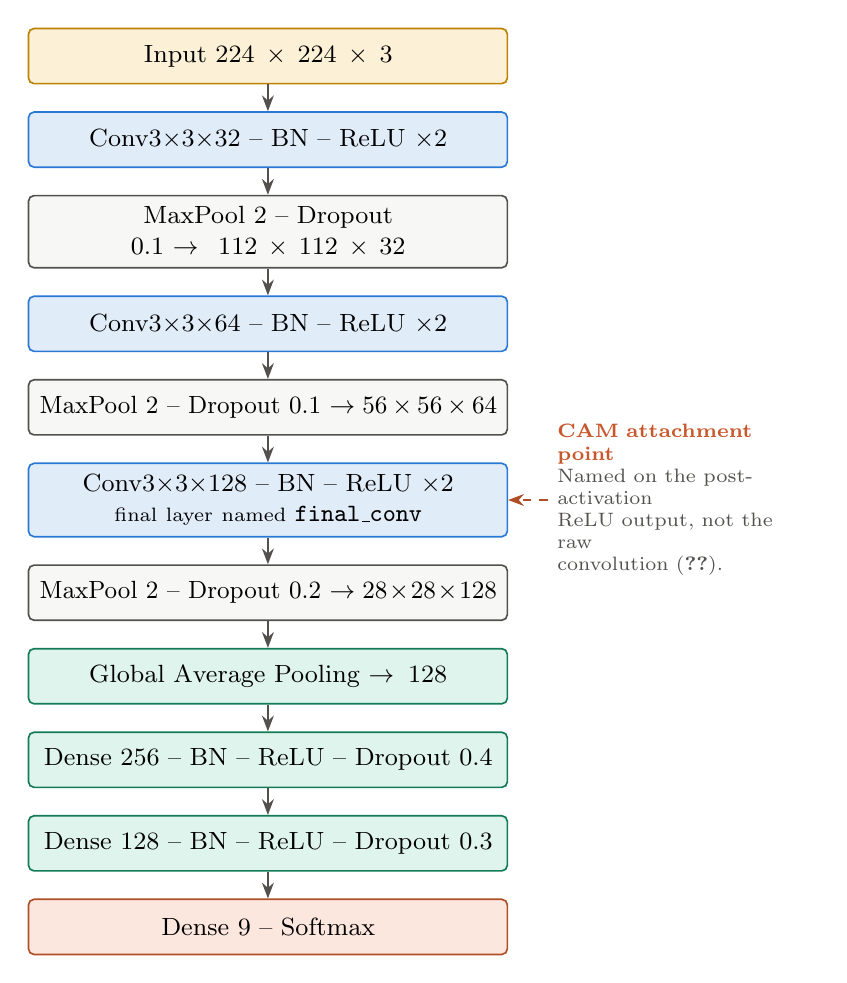
\begin{tikzpicture}[
  node distance=3.4mm,
  every node/.style={font=\small, align=center},
  blk/.style={draw=inkblack, rounded corners=2pt, minimum height=7mm,
              text width=58mm, inner sep=4pt, line width=0.6pt},
  conv/.style={blk, fill=honestblue!14, draw=honestblue},
  pool/.style={blk, fill=panelbg, draw=mutedgray, text width=58mm},
  head/.style={blk, fill=goodgreen!14, draw=goodgreen!70!black},
  tag/.style={font=\scriptsize\color{mutedgray}, align=left},
]
  \node[blk, fill=amberwarn!16, draw=amberwarn!80!black] (in) {Input $224\times224\times3$};
  \node[conv, below=of in] (c1) {Conv$3{\times}3{\times}32$ -- BN -- ReLU $\times 2$};
  \node[pool, below=of c1] (p1) {MaxPool 2 -- Dropout 0.1 $\rightarrow 112\times112\times32$};
  \node[conv, below=of p1] (c2) {Conv$3{\times}3{\times}64$ -- BN -- ReLU $\times 2$};
  \node[pool, below=of c2] (p2) {MaxPool 2 -- Dropout 0.1 $\rightarrow 56\times56\times64$};
  \node[conv, below=of p2] (c3) {Conv$3{\times}3{\times}128$ -- BN -- ReLU $\times 2$ \\ \scriptsize final layer named \code{final\_conv}};
  \node[pool, below=of c3] (p3) {MaxPool 2 -- Dropout 0.2 $\rightarrow 28\times28\times128$};
  \node[head, below=of p3] (gap) {Global Average Pooling $\rightarrow 128$};
  \node[head, below=of gap] (fc1) {Dense 256 -- BN -- ReLU -- Dropout 0.4};
  \node[head, below=of fc1] (fc2) {Dense 128 -- BN -- ReLU -- Dropout 0.3};
  \node[blk, fill=leakyorange!16, draw=leakyorange!75!black, below=of fc2] (out) {Dense 9 -- Softmax};

  \foreach \a/\b in {in/c1, c1/p1, p1/c2, c2/p2, p2/c3, c3/p3, p3/gap, gap/fc1, fc1/fc2, fc2/out}
    \draw[-{Stealth[length=2mm]}, line width=0.8pt, color=mutedgray] (\a) -- (\b);

  \node[tag, right=5mm of c3, text width=32mm] (camnote)
    {\textcolor{leakyorange!85!black}{\textbf{CAM attachment point}}\\
     Named on the post-activation \\ ReLU output, not the raw \\ convolution
     (\cref{sec:cam-attachment}).};
  \draw[-{Stealth[length=2mm]}, line width=0.8pt, dashed, color=leakyorange!75!black]
        (camnote.west) -- (c3.east);
\end{tikzpicture}
\caption{\LXNet{} architecture. All convolutions use \code{use\_bias=False}
since batch normalisation makes an explicit bias redundant. Every layer is
named so the network graph is addressable by name for interpretability and
testing.}
\label{fig:lxnet-arch}
\end{figure}

\subsection{Global Average Pooling Is the Parameter Budget}

The single architectural decision responsible for \LXNet{}'s parameter count
is using global average pooling instead of flattening before the classifier
head. Flattening the final $28\times28\times128$ feature map and feeding it
to a 256-unit dense layer would cost
$28 \times 28 \times 128 \times 256 = 25{,}690{,}112$ weights on that one
layer alone --- more than 70 times the entire network's actual parameter
count. Global average pooling collapses each of the 128 channels to a single
scalar first, so the same dense layer costs $128 \times 256 = 32{,}768$
weights instead.

\section{Transfer-Learning Baselines}

Three ImageNet-pretrained backbones are wired behind an identical classifier
head (global average pooling, Dense-256-ReLU, Dropout 0.4, Dense-9-softmax),
frozen by default (\code{trainable\_backbone=False}). The backbone is frozen
because the comparison of interest is \emph{\LXNet{} trained from scratch}
against \emph{the standard "pretrained backbone plus a new head"} recipe most
practitioners would actually reach for --- and a fair comparison needs an
identical head shape across all four models, which \code{build\_baseline}
enforces structurally rather than by convention.

\begin{table}[h]
\centering
\small
\begin{tabular}{@{}lrlll@{}}
\toprule
\textbf{Model} & \textbf{Parameters} & \textbf{Pretrained} & \textbf{Backbone
trainable} & \textbf{Learning rate} \\
\midrule
\LXNet{} & 356{,}585 & No (from scratch) & --- & $1\times10^{-3}$ \\
DenseNet201 & 18{,}816{,}073 & ImageNet & Frozen & $1\times10^{-4}$ \\
InceptionV3 & 22{,}329{,}641 & ImageNet & Frozen & $1\times10^{-4}$ \\
ResNet50V2 & 24{,}091{,}657 & ImageNet & Frozen & $1\times10^{-4}$ \\
\bottomrule
\end{tabular}
\caption{All four models, as instantiated by \texttt{lxnet.models.build\_model}.
Parameter counts are measured via \texttt{model.count\_params()} at train
time and asserted by \texttt{tests/test\_models.py} against a 500{,}000
budget for \LXNet{} (the reference paper's claim is $\approx$0.35\,M).}
\label{tab:model-params}
\end{table}

\LXNet{} trains at $10\times$ the learning rate of the baselines because it
trains every weight from a random initialisation, while the baselines are
only fitting a small randomly-initialised head on top of frozen, already
well-conditioned ImageNet features --- a higher rate on the frozen-backbone
models would risk destabilising the head before it has had a chance to
converge against fixed features.

\section{The CAM Attachment Point}
\label{sec:cam-attachment}

The final convolutional block's activation layer is explicitly named
\code{final\_conv}, and this is not cosmetic --- it is the layer every
interpretability method in \cref{ch:xai} attaches to, and its position in the
Conv $\to$ BatchNorm $\to$ Activation sequence matters:

\begin{itemize}
\item the \textbf{raw convolution output} is pre-BatchNorm, so its
  per-channel scale is arbitrary and not comparable across channels;
\item it is also \textbf{signed}, so a channel's negative activations survive
  into a weighted sum in a way Grad-CAM's formulation does not account for;
\item the \textbf{post-activation} (post-ReLU) output is what Grad-CAM
  \cite{selvaraju2017} is defined over: non-negative, batch-normalised, and
  directly comparable across channels.
\end{itemize}

\code{xai.\_feature\_layer} raises a explicit \code{ValueError} if the
requested layer name is not found in the model, rather than silently falling
back to a default --- an earlier version of this code returned the default
unchecked, which meant a model missing the expected attachment point failed
deep inside \code{model.get\_layer} with no indication of why.

% ===========================================================================
\chapter{Training Methodology}
\label{ch:training}

\section{Optimisation Configuration}

\begin{table}[h]
\centering
\small
\begin{tabular}{@{}ll@{}}
\toprule
\textbf{Setting} & \textbf{Value} \\
\midrule
Optimiser & Adam \\
Loss & Sparse categorical cross-entropy \\
Batch size & 32 \\
Max epochs & 40 \\
Early stopping & monitor \code{val\_loss}, patience 8, \code{restore\_best\_weights=True} \\
LR schedule & \code{ReduceLROnPlateau}, monitor \code{val\_loss}, factor 0.5, patience 2, min LR $1\times10^{-6}$ \\
Checkpointing & best \code{val\_loss} only, weights only \\
Seed & 42 (\code{tf.keras.utils.set\_random\_seed}) \\
\bottomrule
\end{tabular}
\caption{Training configuration, identical across all four models and both
split protocols. Only the per-model learning rate differs
(\cref{tab:model-params}).}
\label{tab:train-config}
\end{table}

\section{Hold-Out Training}

\code{train.train\_once} builds fresh \code{tf.data} pipelines for the
train, validation and test index arrays, fits with the callback stack in
\cref{tab:train-config}, and scores the fitted model on the held-out test
indices exactly once. \code{tf.keras.backend.clear\_session()} is called
before every model build so that successive runs in the same process (four
models per hold-out pass, then up to five more per cross-validation fold) do
not accumulate graph state across models with different architectures.

\section{Cross-Validation and the Early-Stopping Leak}
\label{sec:carve-validation}

$k$-fold cross-validation raises a subtler correctness problem than the
train/test split does. Early stopping with \code{restore\_best\_weights}
does not simply train for a fixed number of epochs --- it trains for up to
40 epochs and \emph{keeps whichever epoch's weights scored best on the
validation set it is watching}. If that validation set is the same fold
being reported as the cross-validation score, the reported number is not
"the model's accuracy" but "the maximum of the model's accuracy over up to
40 draws" --- a systematic optimistic bias that grows with the patience
budget.

\code{train.\_carve\_validation} avoids this by splitting each fold's
\emph{training} rows a second time, stratified by class, into an inner
training set and a small early-stopping monitor (15\% by default, with at
least one example per class held back where the class is large enough). The
held-out fold that is actually scored is never touched until the model has
already stopped training on it.

\begin{lstlisting}[caption={The inner train/monitor split that keeps
early-stopping honest (\texttt{lxnet/train.py}).}, label=lst:carve]
def _carve_validation(
    idx: np.ndarray, labels: np.ndarray, seed: int, fraction: float = 0.15
) -> tuple[np.ndarray, np.ndarray]:
    """Split fold-training rows into (train, early-stopping monitor), stratified.

    ponytail: carves by row, not by perceptual group, so a near-duplicate may
    straddle the inner boundary. That only blunts the stopping-epoch choice --
    the reported score comes from the outer fold, which stays group-clean.
    Carve by group if the stopping epoch ever looks systematically late.
    """
\end{lstlisting}

\begin{debtbox}
\code{\_carve\_validation} splits by individual cache row, not by perceptual
group, so a near-duplicate pair can straddle the inner train/monitor boundary
within a fold. This is deliberately left as-is: the boundary it affects only
influences \emph{which epoch} early stopping selects, not the score that gets
reported --- the outer, scored fold remains perceptual-group-clean regardless.
The upgrade path, if the stopping epoch is ever observed to be systematically
too late (a symptom of the monitor being easier than it should be), is to
carve by group using the same machinery as \cref{sec:group-aware-split}.
\end{debtbox}

Oversampling is applied \emph{after} this inner carve, and only to the inner
training rows --- the same ordering constraint from
\cref{sec:balance-order}, applied one level deeper so that a duplicated
minority-class row cannot appear in both the inner training set and the
monitor set within a single fold.

\section{The GPU Guard}
\label{sec:gpu-guard}

TensorFlow 2.10 on Windows locates the CUDA runtime through the active
Conda environment's \texttt{Library/bin} directory on \texttt{PATH}, which
\code{conda activate} sets up. Invoking the environment's
\texttt{python.exe} by an absolute path (for example, from a scheduled task
or an IDE run configuration that does not source the activation script)
silently falls back to CPU --- training still runs, still produces a
model, and turns a 40-minute job into an overnight one with no error message
anywhere in the log.

\code{train.main} refuses to start training on CPU unless
\code{-{}-allow-cpu} is passed explicitly:

\begin{lstlisting}[caption={Fail fast rather than discover a CPU fallback the
next morning (\texttt{lxnet/train.py}).}, label=lst:gpuguard]
if not gpus and not args.allow_cpu:
    raise SystemExit(
        "no GPU visible to TensorFlow -- refusing to train on CPU.\n"
        "Activate the env (`conda activate lxnet`) so CUDA is on PATH, "
        "or pass --allow-cpu."
    )
\end{lstlisting}

This is a case where the lazy failure mode (silently doing the slow thing)
is strictly worse than the loud one: a training run that aborts in the first
second is a two-second fix, while one that silently spends nine hours on CPU
is discovered only when someone checks on it.

\section{Determinism and Seeding}

A single seed (default 42) drives every source of randomness in a run:
\code{tf.keras.utils.set\_random\_seed} for the model's weight
initialisation and TensorFlow-internal shuffling, and
\code{numpy.random.default\_rng(seed)} for every split, grouping-tie-break
and oversampling decision in \code{data.py} and \code{train.py}.
Cross-validation folds derive per-fold seeds as \code{seed + fold} for the
inner carve and oversampling steps, so each fold's inner split is
reproducible but not identical across folds. Full bit-for-bit reproducibility
across machines is not claimed --- cuDNN convolution algorithms are not
guaranteed deterministic across GPU models and driver versions --- but every
source of randomness under this codebase's control is seeded and logged.

% ===========================================================================
\chapter{Evaluation Methodology}
\label{ch:evaluation}

\section{Macro-Averaged Metrics}

Every reported precision, recall and F1 score in this system is macro-averaged:
computed independently per class, then averaged with equal weight regardless
of class support. \Cref{tab:class-dist} showed why this is not a stylistic
choice --- Normal (1{,}340 images) outnumbers Chest Changes (544 images) by
2.5:1, and a micro-averaged (support-weighted) metric would let a model that
neglects the smallest classes still post a respectable headline number,
because those classes contribute little to the weighted total. Macro
averaging forces every class's performance to matter equally to the reported
score, which is the property an evaluator actually wants when the classes
are not clinically interchangeable.

\code{evaluate.compute\_metrics} wraps
\code{sklearn.metrics.precision\_recall\_fscore\_support} with
\code{average="macro"} and \code{zero\_division=0} (so a class with zero
predicted or zero true instances contributes 0 rather than raising or
silently excluding itself), and always returns the full confusion matrix
alongside the scalar metrics --- every per-class table and confusion-matrix
figure in \cref{ch:results} is derived from this one matrix, not
recomputed independently.

\section{Cross-Fold Summarisation}

\code{evaluate.summarise\_folds} computes the mean and population standard
deviation of every numeric metric across a list of per-fold result
dictionaries, skipping non-numeric fields automatically (so it can be handed
a fold's full metrics dictionary, including the confusion matrix, without
special-casing which keys are summarisable).

\section{Paired Significance Testing}

Comparing two models' cross-validation scores is a paired-samples problem:
both models are scored on the \emph{same} folds, so the correct test compares
per-fold differences rather than treating the two score distributions as
independent samples. With only five folds, assuming those differences are
normally distributed is not defensible, so
\code{evaluate.wilcoxon\_compare} uses the Wilcoxon signed-rank test
\cite{wilcoxon1945} --- non-parametric, and appropriate for small paired
samples.

\begin{lstlisting}[caption={Paired, non-parametric comparison across
cross-validation folds (\texttt{lxnet/evaluate.py}).}, label=lst:wilcoxon]
def wilcoxon_compare(a, b, alpha: float = ALPHA) -> dict:
    differences = a - b
    if np.allclose(differences, 0):
        # scipy raises on an all-zero difference vector;
        # the answer is "no effect".
        return {"statistic": 0.0, "p_value": 1.0,
                "significant": False, "median_difference": 0.0}
    statistic, p_value = wilcoxon(a, b)
    return {
        "statistic": float(statistic), "p_value": float(p_value),
        "significant": bool(p_value < alpha),
        "median_difference": float(np.median(differences)),
    }
\end{lstlisting}

The all-zero-difference guard is not a hypothetical edge case: SciPy's
Wilcoxon implementation raises on a rank-degenerate input, and two identical
score vectors is exactly the input a unit test would use to check "no
difference reports as no difference" --- the function needs to handle that
input correctly, not just the well-behaved ones. As reported in
\cref{sec:significance}, only \LXNet{} was cross-validated in the measured
run, so this comparison currently has one populated arm.

% ===========================================================================
\chapter{Experimental Results}
\label{ch:results}

All results in this chapter are measured, not projected: both the
group-aware and random arms were trained end-to-end with the configuration
in \cref{tab:train-config}, and every figure below is generated directly
from the resulting \texttt{results.json} by \code{lxnet.report} --- none is
hand-drawn (\cref{sec:repro-record}).

\section{Headline Finding}

Under a random split, 40.4\% of test images have a near-duplicate in the
training set; under the group-aware split, none do. \LXNet{} scores 92.9\% on
the group-aware test set against 95.4\% on the random split --- a 2.5
percentage-point gain that is attributable entirely to leakage, since both
numbers come from the same model, the same weights, and the same
preprocessing. The strongest model overall, on the honest split, is
ResNet50V2 at 98.5\%.

\begin{figure}[htbp]
\centering
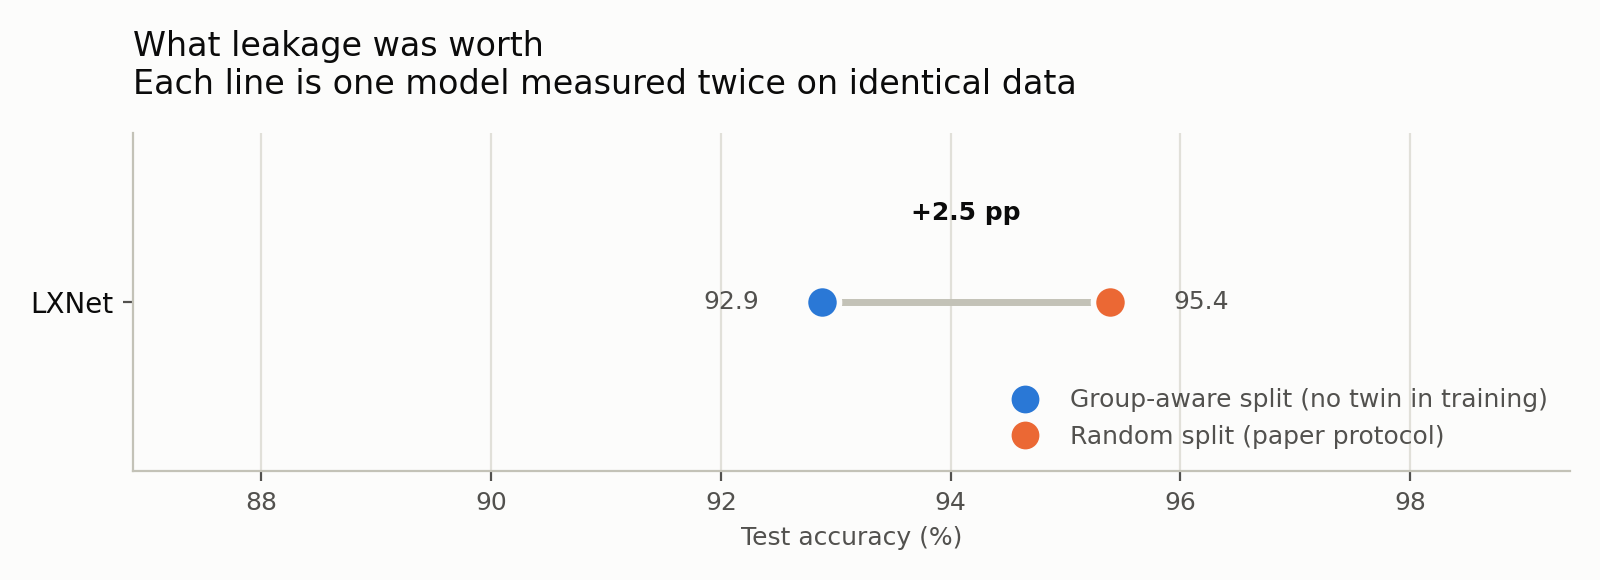
\includegraphics[width=0.92\textwidth]{fig_gap.png}
\caption{Accuracy under each split protocol, per model. Each pair of points
is one model measured twice on identical data; the only variable is whether
a re-saved copy of a training image was allowed into the test set.}
\label{fig:gap}
\end{figure}

\section{Hold-Out Comparison}

\begin{table}[h]
\centering
\small
\resizebox{\linewidth}{!}{%
\begin{tabular}{@{}lrrrrr@{}}
\toprule
\textbf{Model} & \textbf{Params} & \textbf{Group-aware acc.\ (\%)} &
\textbf{Group-aware F1} & \textbf{Random-split acc.\ (\%)} & \textbf{Inflation (pp)} \\
\midrule
ResNet50V2 & 24.09\,M & 98.5 & 0.988 & --- & --- \\
DenseNet201 & 18.82\,M & 97.4 & 0.980 & --- & --- \\
InceptionV3 & 22.33\,M & 94.8 & 0.953 & --- & --- \\
\LXNet{} & 357\,K & 92.9 & 0.938 & 95.4 & +2.5 \\
\bottomrule
\end{tabular}%
}
\caption{Hold-out comparison across both split protocols. Only \LXNet{} was
trained under the random-split arm (\cref{sec:significance}); the backbones
were run group-aware only, for training-time reasons
(\cref{tab:training-cost}).}
\label{tab:holdout}
\end{table}

\begin{table}[h]
\centering
\small
\begin{tabular}{@{}lrrrr@{}}
\toprule
\textbf{Model} & \textbf{Accuracy} & \textbf{Precision (macro)} &
\textbf{Recall (macro)} & \textbf{Macro-F1} \\
\midrule
ResNet50V2 & 98.50 & 98.70 & 99.02 & 0.9885 \\
DenseNet201 & 97.39 & 97.77 & 98.20 & 0.9797 \\
InceptionV3 & 94.78 & 95.13 & 95.69 & 0.9534 \\
\LXNet{} & 92.88 & 93.16 & 95.06 & 0.9382 \\
\bottomrule
\end{tabular}
\caption{Every headline metric, group-aware hold-out, all percentages except
Macro-F1.}
\label{tab:full-metrics}
\end{table}

\section{Does the Small Model Keep Up?}

The reference paper's central claim is that $\approx$0.35\,M parameters can
match backbones 50--70$\times$ larger. That claim is only testable on a split
where the models can actually be told apart --- under enough leakage, every
model's accuracy compresses toward the ceiling the dataset allows, and the
parameter-efficiency argument becomes unfalsifiable.

\begin{figure}[htbp]
\centering
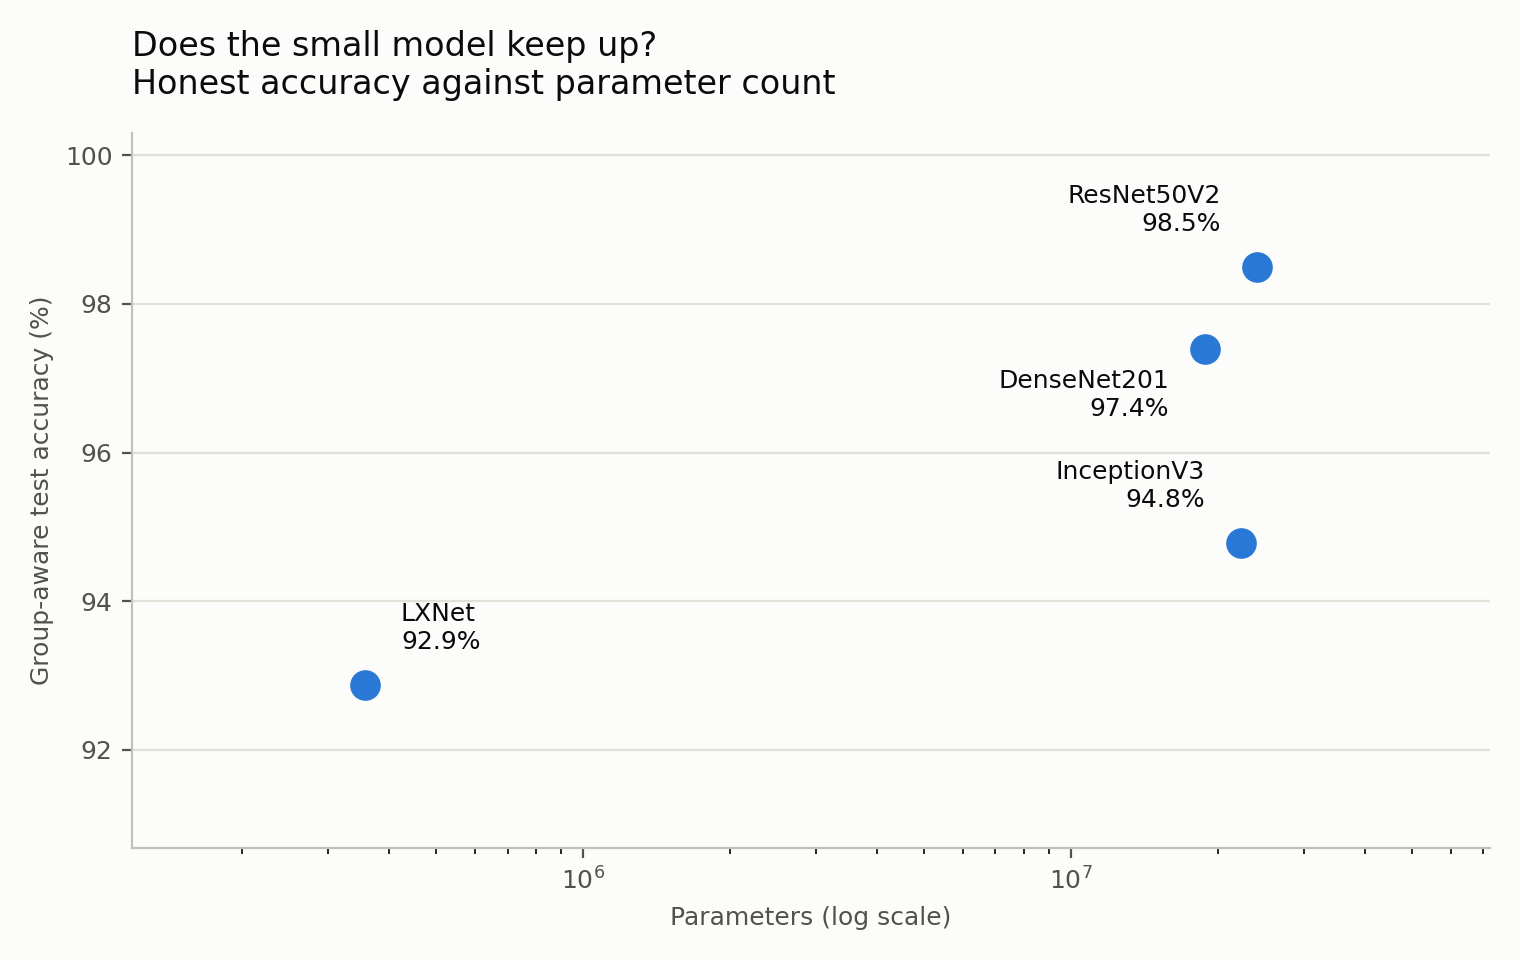
\includegraphics[width=0.85\textwidth]{fig_efficiency.png}
\caption{Group-aware test accuracy against parameter count (log scale).
\LXNet{} trails the largest backbone by 5.6 percentage points at
$1/67$\textsuperscript{th} the parameter count.}
\label{fig:efficiency}
\end{figure}

\begin{figure}[htbp]
\centering
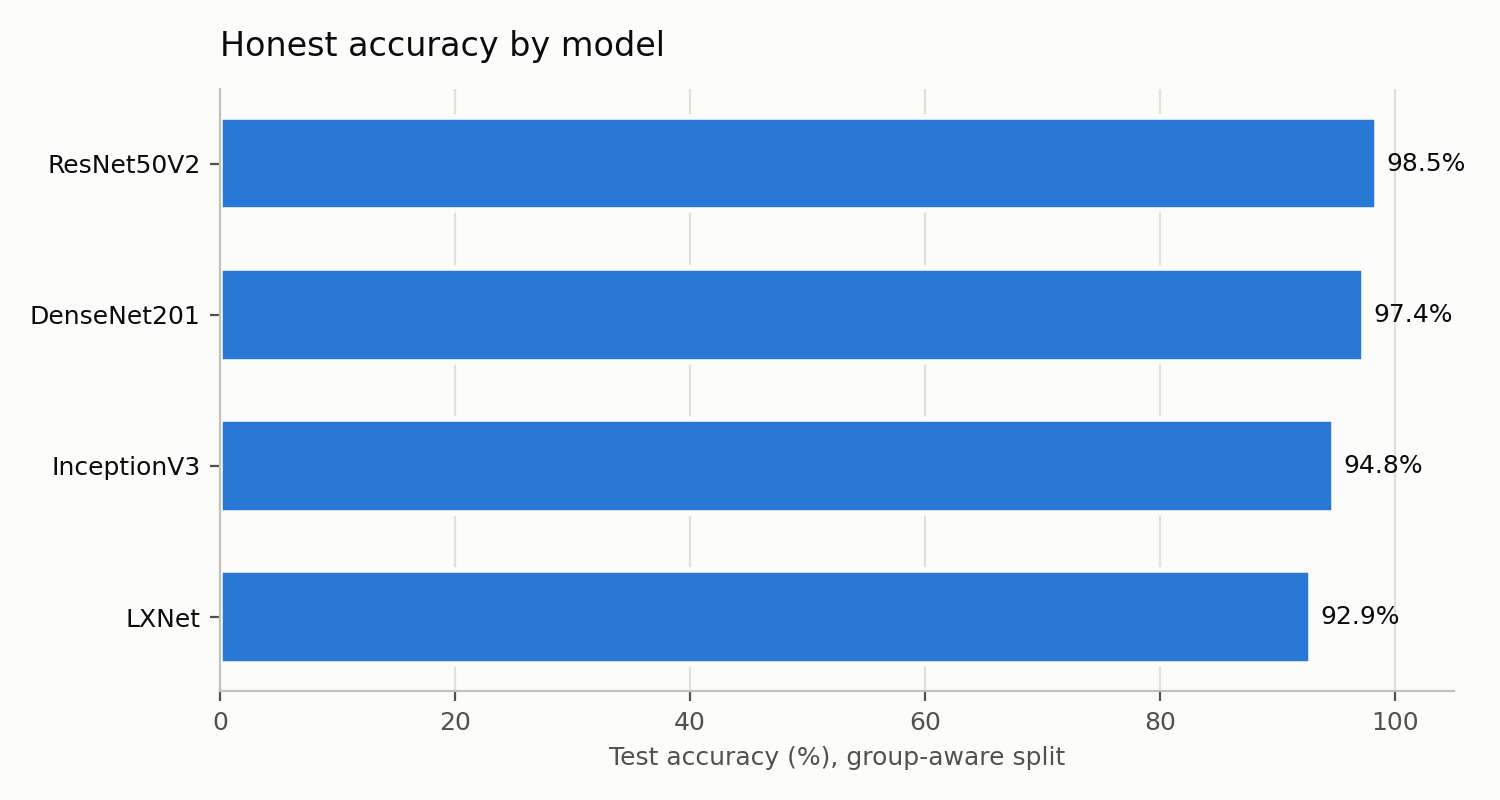
\includegraphics[width=0.82\textwidth]{fig_accuracy_by_model.png}
\caption{Honest (group-aware) accuracy by model, ranked.}
\label{fig:acc-by-model}
\end{figure}

The trade is explicit: \LXNet{} gives up 5.6 percentage points of accuracy to
ResNet50V2 and returns 260.5 accuracy points per million parameters against
ResNet50V2's 4.1 --- a 63$\times$ improvement in the efficiency metric
(\cref{tab:training-cost}). Whether that trade is worth making depends
entirely on the deployment target: a datacentre inference service has little
reason to prefer \LXNet{} over ResNet50V2, while a CPU-only edge device in a
clinic without GPU access may not have the option to run the larger model at
all.

\section{Cross-Validation}

\begin{figure}[htbp]
\centering
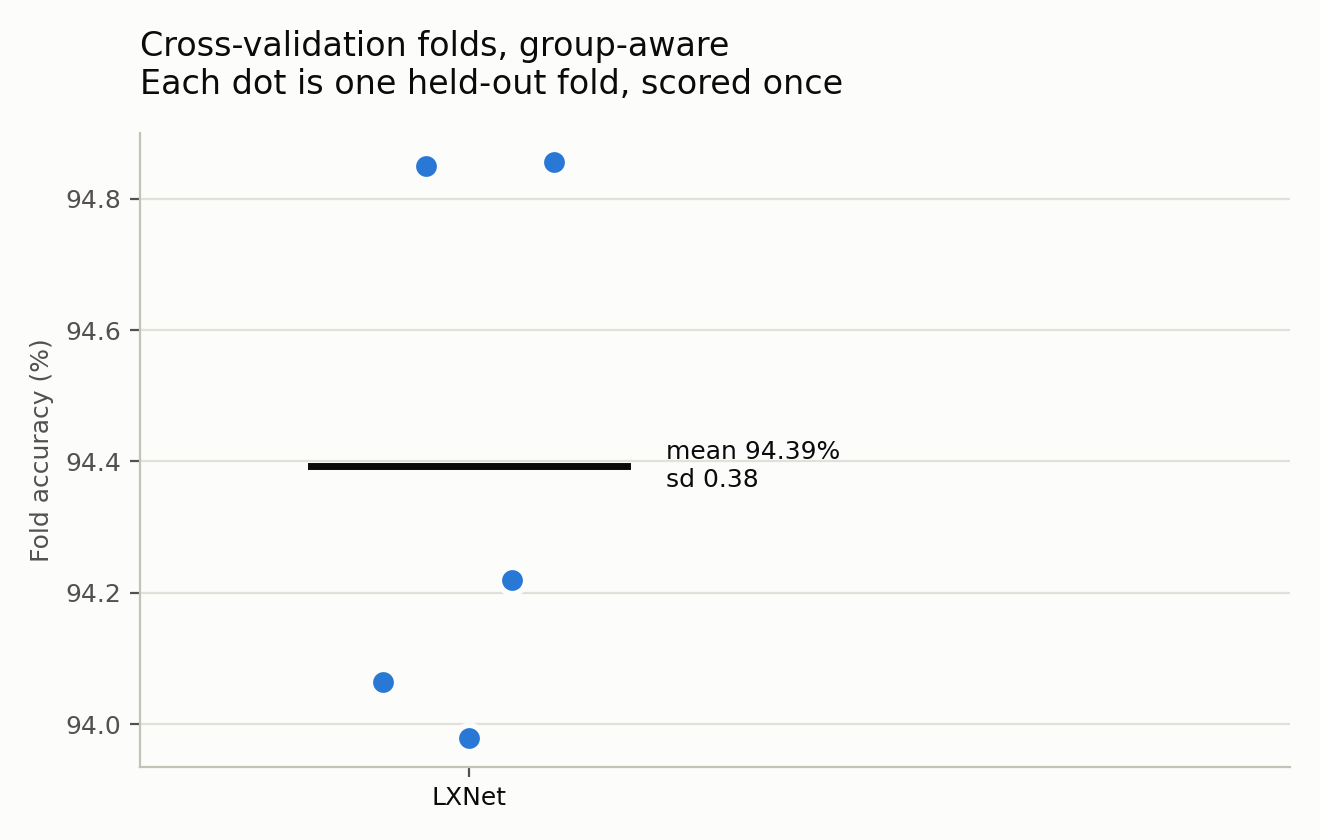
\includegraphics[width=0.75\textwidth]{fig_cv_folds.png}
\caption{Per-fold accuracy, 5-fold group-aware cross-validation, \LXNet{}
only.}
\label{fig:cv-folds}
\end{figure}

\begin{table}[h]
\centering
\small
\begin{tabular}{@{}lrrr@{}}
\toprule
\textbf{Model} & \textbf{Folds} & \textbf{Accuracy (\%)} & \textbf{Macro-F1} \\
\midrule
\LXNet{} (group-aware) & 5 & $94.39 \pm 0.38$ & 0.9504 \\
\LXNet{} (random) & 5 & $95.14 \pm 1.55$ & --- \\
\bottomrule
\end{tabular}
\caption{Cross-validation accuracy, both split protocols, identical model and
preprocessing. Note the standard deviation: leakage does not only inflate the
mean, it more than quadruples the fold-to-fold spread, because how much a
random-split fold scores depends on how many of its images happen to have a
twin sitting in that fold's training portion.}
\label{tab:cv}
\end{table}

Each fold's early-stopping monitor is carved out of that fold's
\emph{training} rows (\cref{sec:carve-validation}), so the reported fold is
touched exactly once, at scoring time, and never influences which epoch's
weights are restored.

\section{Where the Errors Are}

\begin{figure}[htbp]
\centering
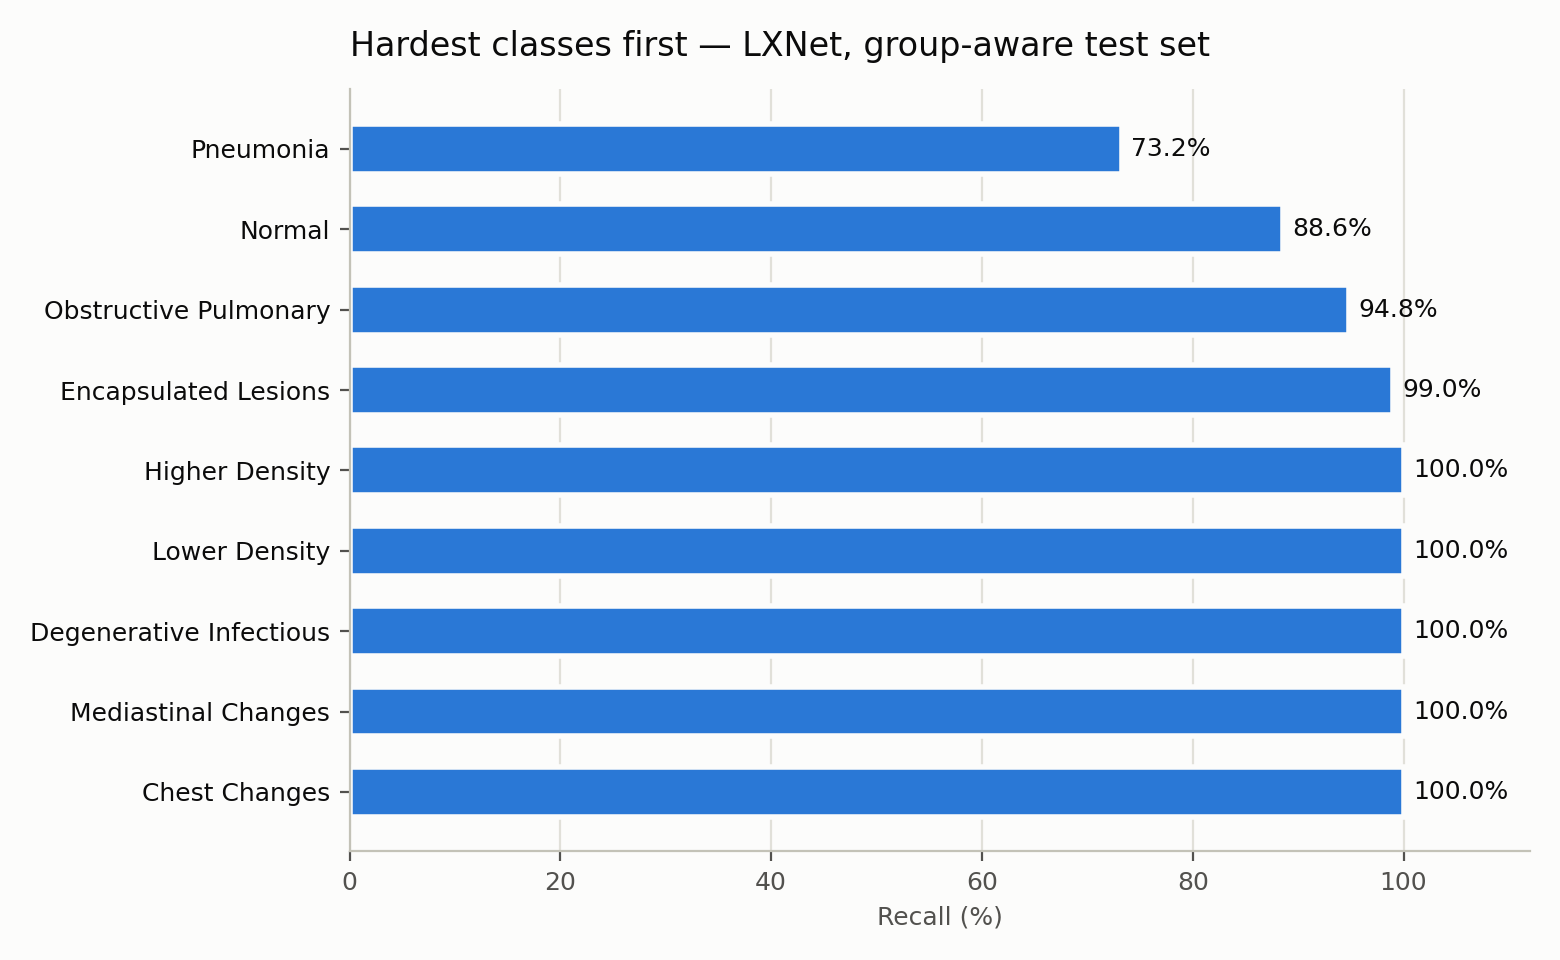
\includegraphics[width=0.85\textwidth]{fig_per_class.png}
\caption{Per-class recall, \LXNet{}, group-aware test set, hardest classes
first.}
\label{fig:per-class}
\end{figure}

\begin{table}[h]
\centering
\small
\begin{tabular}{@{}lrrrr@{}}
\toprule
\textbf{Class} & \textbf{Precision} & \textbf{Recall} & \textbf{F1} & \textbf{Support} \\
\midrule
Normal & 93.7 & 88.6 & 0.910 & 201 \\
Pneumonia & 93.5 & 73.2 & 0.821 & 157 \\
Higher Density & 88.5 & 100.0 & 0.939 & 100 \\
Lower Density & 96.8 & 100.0 & 0.984 & 91 \\
Obstructive Pulmonary & 94.8 & 94.8 & 0.948 & 96 \\
Degenerative Infectious & 83.0 & 100.0 & 0.907 & 88 \\
Encapsulated Lesions & 91.4 & 99.0 & 0.950 & 97 \\
Mediastinal Changes & 96.7 & 100.0 & 0.983 & 88 \\
Chest Changes & 100.0 & 100.0 & 1.000 & 79 \\
\bottomrule
\end{tabular}
\caption{Per-class detail, \LXNet{}, group-aware test set.}
\label{tab:per-class-lxnet}
\end{table}

\begin{table}[h]
\centering
\small
\begin{tabular}{@{}lrrrr@{}}
\toprule
\textbf{Class} & \textbf{ResNet50V2} & \textbf{DenseNet201} & \textbf{InceptionV3} & \textbf{\LXNet{}} \\
\midrule
Normal & 97.5 & 94.5 & 96.0 & 88.6 \\
Pneumonia & 93.6 & 92.4 & 82.2 & 73.2 \\
Higher Density & 100.0 & 100.0 & 100.0 & 100.0 \\
Lower Density & 100.0 & 100.0 & 97.8 & 100.0 \\
Obstructive Pulmonary & 100.0 & 100.0 & 93.8 & 94.8 \\
Degenerative Infectious & 100.0 & 100.0 & 96.6 & 100.0 \\
Encapsulated Lesions & 100.0 & 96.9 & 94.8 & 99.0 \\
Mediastinal Changes & 100.0 & 100.0 & 100.0 & 100.0 \\
Chest Changes & 100.0 & 100.0 & 100.0 & 100.0 \\
\bottomrule
\end{tabular}
\caption{Recall by class, every model, group-aware test set (\%). The
weakest cells --- Pneumonia and Normal --- are the two classes a screening
tool exists to separate, and every model gives up most of its accuracy
there.}
\label{tab:recall-by-class}
\end{table}

Seven of nine classes sit at 94--100\% recall across every model; Pneumonia
and Normal are the outliers, for every architecture tested, not just
\LXNet{}. This pattern --- uniform difficulty concentrated on exactly two
classes across four unrelated architectures --- is treated in
\cref{ch:limitations} as evidence that the easy classes are more likely
separable by acquisition artefacts than by pathology, and is not resolved by
this report.

\subsection{Confusion Matrices}

\begin{figure}[p]
\centering
\begin{subfigure}[t]{0.48\textwidth}
  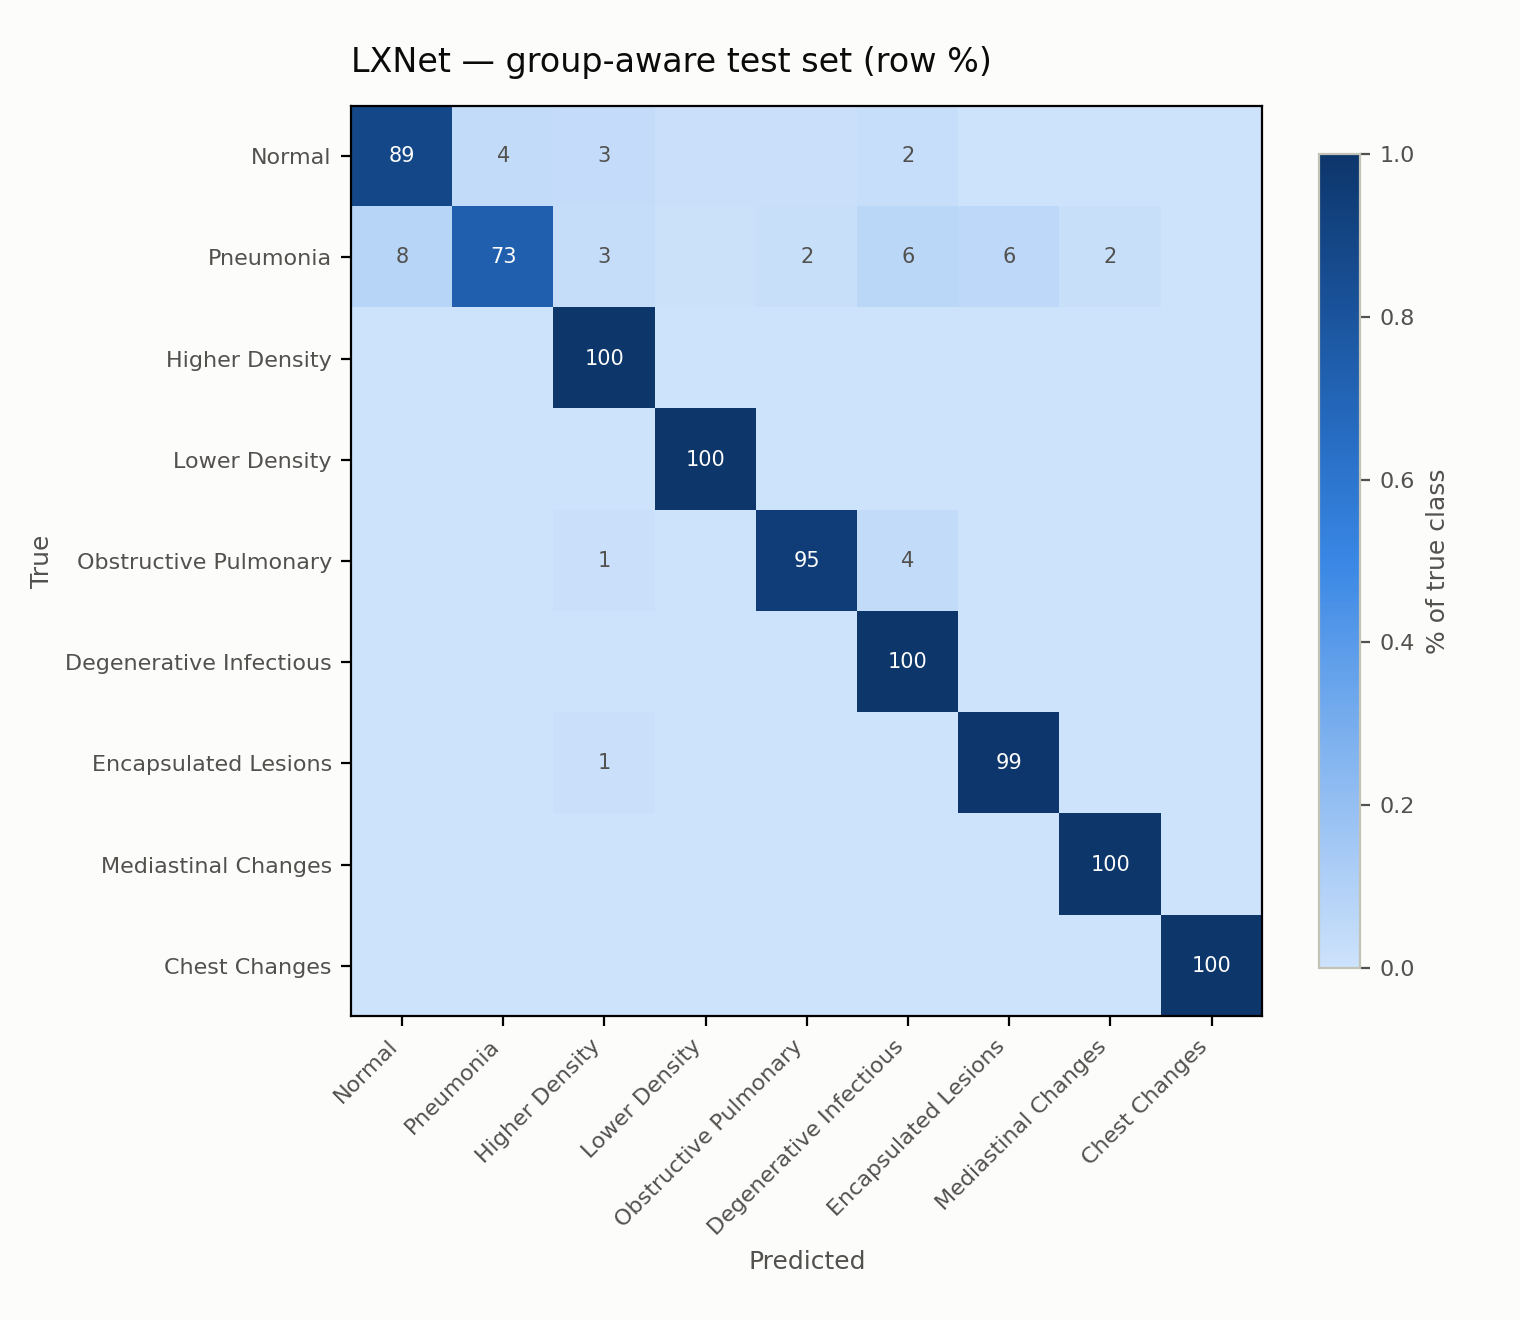
\includegraphics[width=\textwidth]{fig_confusion_LXNet.png}
  \caption{\LXNet{}}
\end{subfigure}\hfill
\begin{subfigure}[t]{0.48\textwidth}
  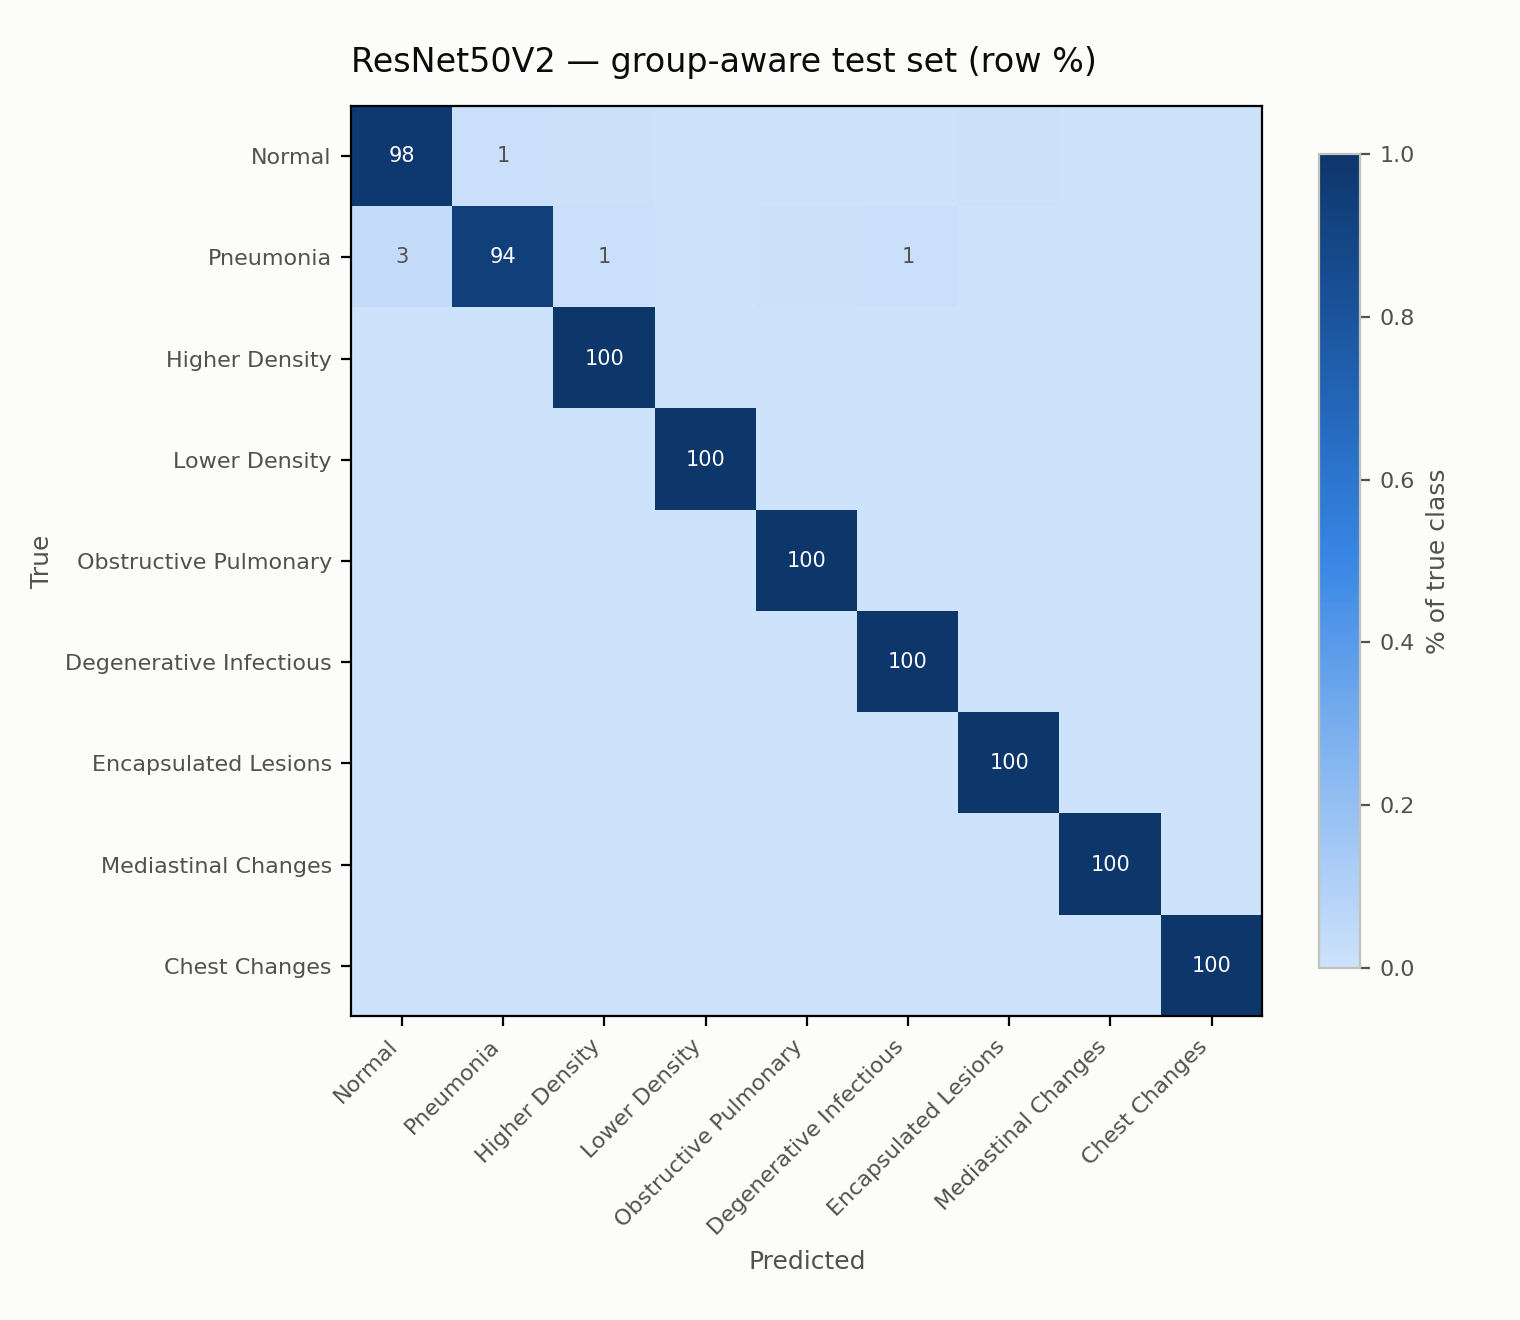
\includegraphics[width=\textwidth]{fig_confusion_ResNet50V2.png}
  \caption{ResNet50V2}
\end{subfigure}

\vspace{0.6cm}
\begin{subfigure}[t]{0.48\textwidth}
  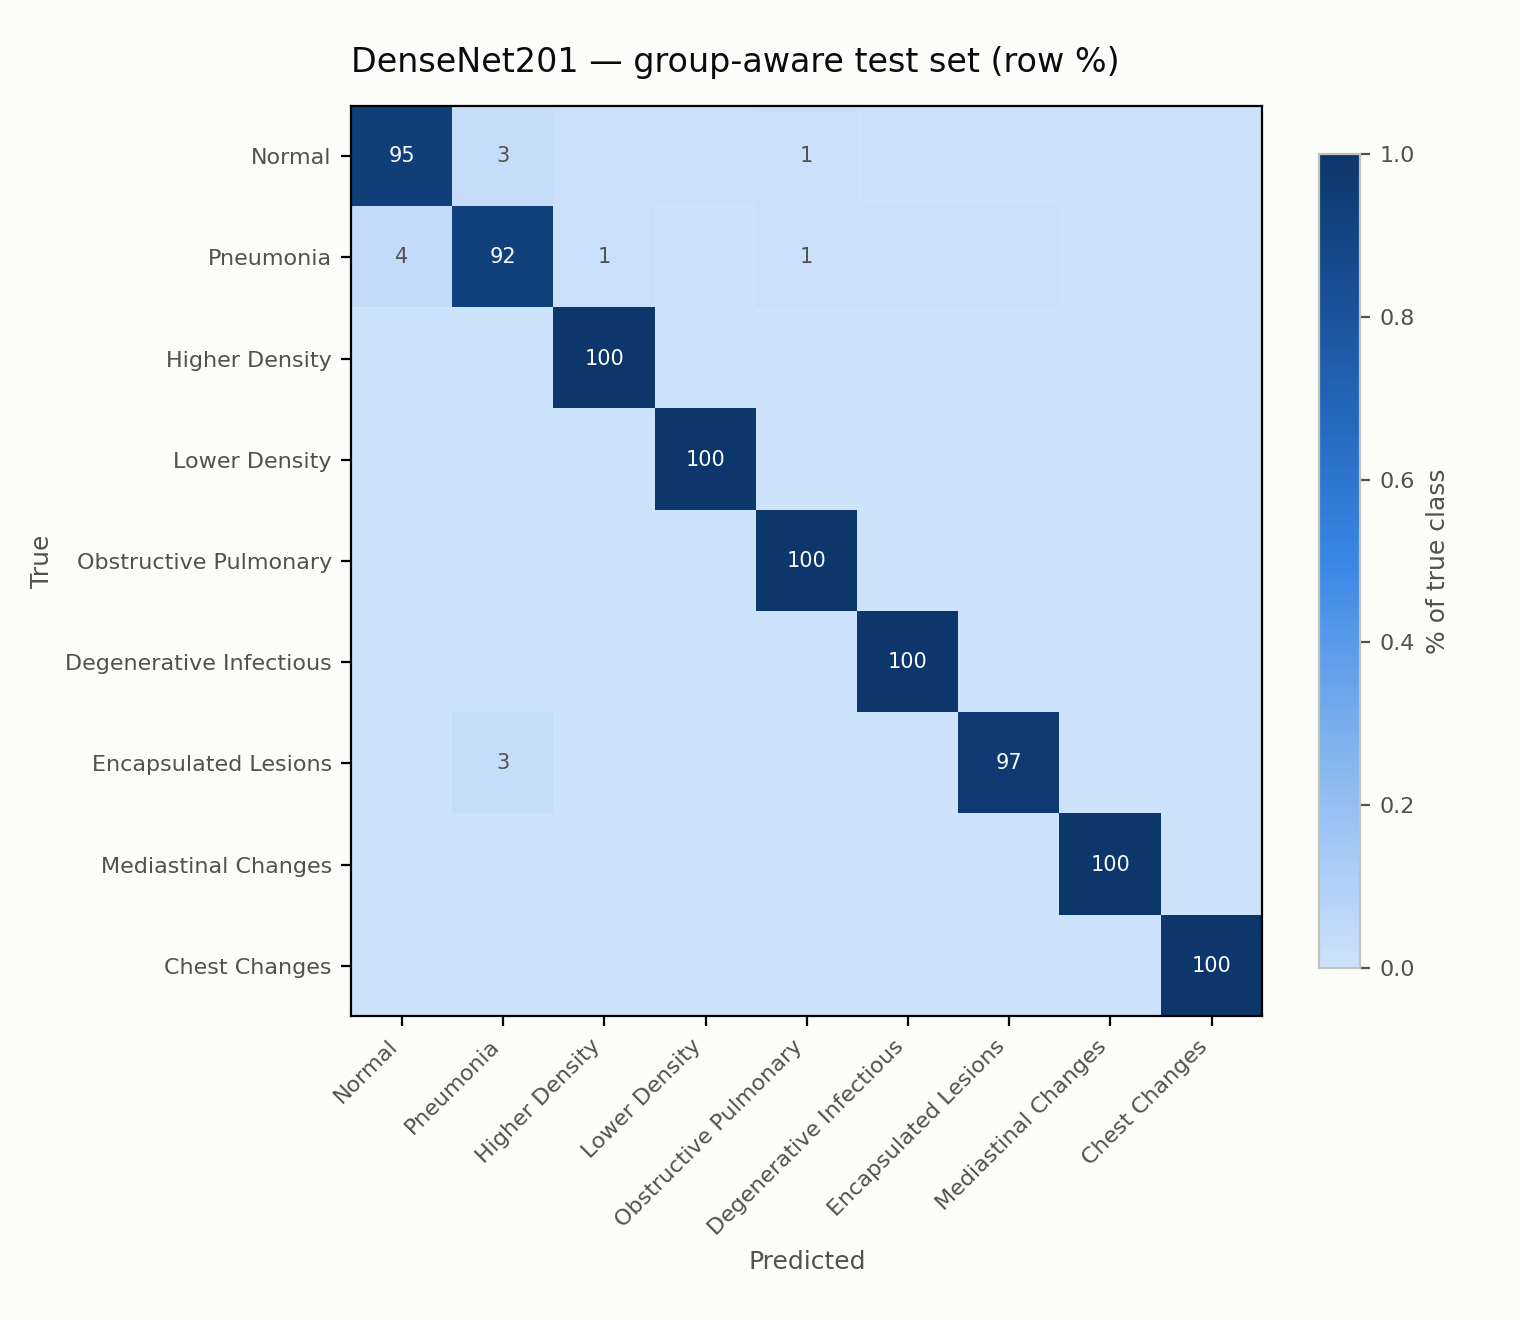
\includegraphics[width=\textwidth]{fig_confusion_DenseNet201.png}
  \caption{DenseNet201}
\end{subfigure}\hfill
\begin{subfigure}[t]{0.48\textwidth}
  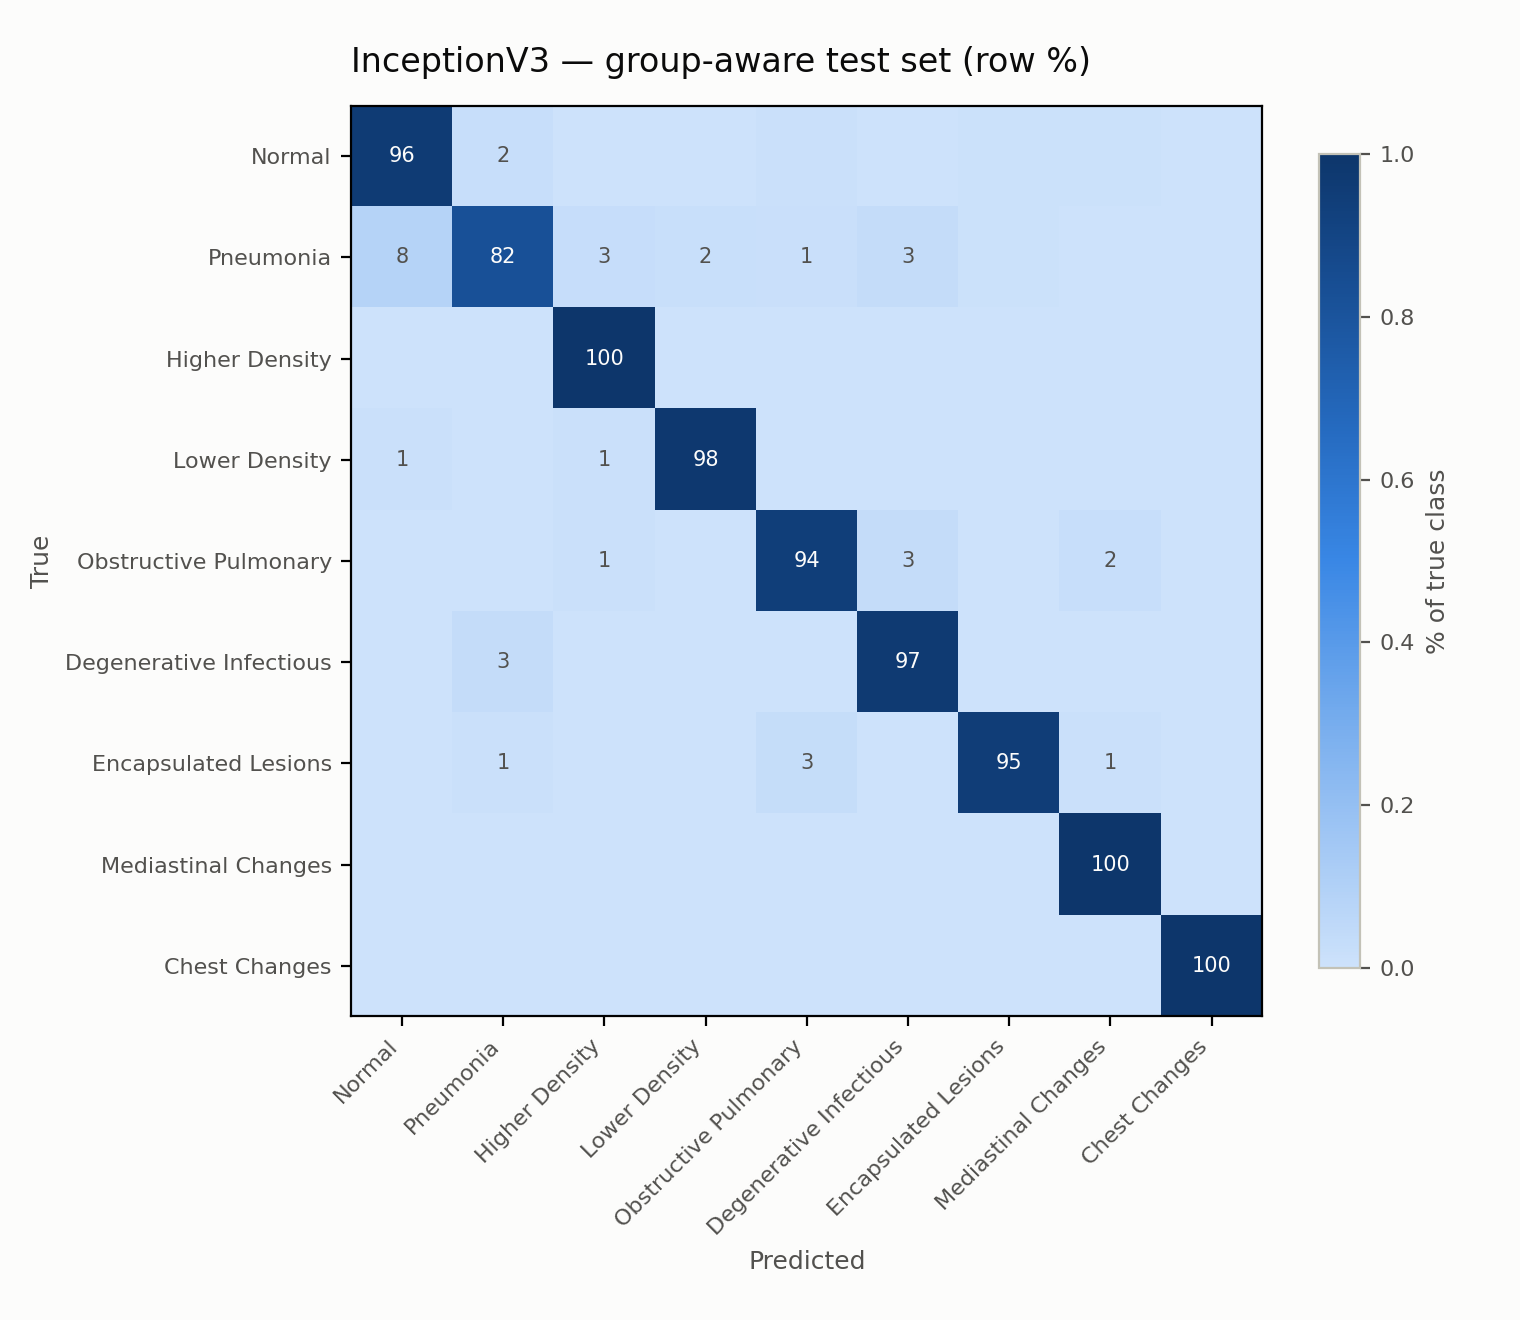
\includegraphics[width=\textwidth]{fig_confusion_InceptionV3.png}
  \caption{InceptionV3}
\end{subfigure}
\caption{Row-normalised confusion matrices, group-aware test set, all four
models. Cell values are percentage of the true class's rows.}
\label{fig:confusion-grid}
\end{figure}

\section{Training Dynamics}

\begin{figure}[htbp]
\centering
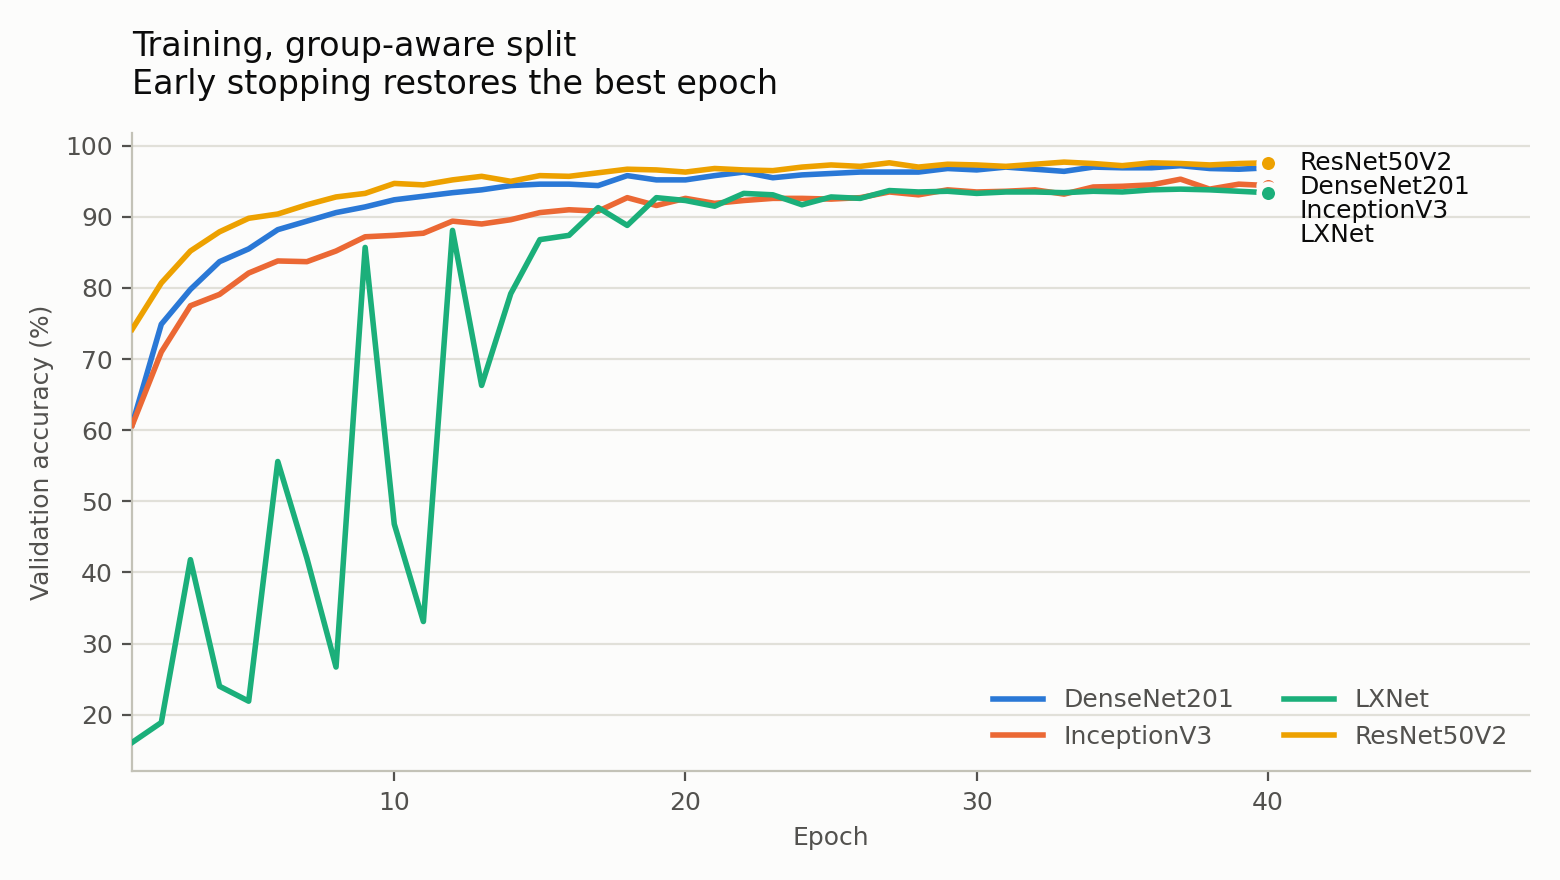
\includegraphics[width=0.85\textwidth]{fig_training.png}
\caption{Validation accuracy per epoch, group-aware split. Early stopping
restores the best-observed epoch per \cref{tab:train-config}.}
\label{fig:training-curves}
\end{figure}

\section{Training Cost}

\begin{table}[h]
\centering
\small
\begin{tabular}{@{}lrrrr@{}}
\toprule
\textbf{Model} & \textbf{Parameters} & \textbf{Epochs run} & \textbf{Wall clock} &
\textbf{Accuracy per M params} \\
\midrule
\LXNet{} & 356{,}585 & 40 & 38m 01s & 260.5 \\
DenseNet201 & 18{,}816{,}073 & 40 & 27m 08s & 5.2 \\
InceptionV3 & 22{,}329{,}641 & 40 & 12m 19s & 4.2 \\
ResNet50V2 & 24{,}091{,}657 & 40 & 12m 54s & 4.1 \\
\bottomrule
\end{tabular}
\caption{Wall-clock training cost, single GPU, group-aware arm. The last
column is deliberately crude (accuracy points per million parameters) but is
the reference paper's argument reduced to one number: \LXNet{} extracts far
more accuracy per parameter than any backbone tested, while still finishing
below all of them in absolute terms. Note that \LXNet{} trains \emph{longer}
in wall-clock time than two of the three frozen-backbone baselines despite
having $50$--$70\times$ fewer parameters --- it is training every weight from
scratch, while the baselines are only fitting a small head on already-frozen
features.}
\label{tab:training-cost}
\end{table}

\section{Significance Testing}
\label{sec:significance}

The Wilcoxon signed-rank comparison in \cref{ch:evaluation} requires two
models scored on the same set of cross-validation folds. In the measured
run, only \LXNet{} was cross-validated --- the three backbones were run
hold-out only, for the training-time reasons visible in
\cref{tab:training-cost} (five-fold cross-validation of ResNet50V2 alone
would cost on the order of an hour of GPU time, repeated per model). This
section is therefore reported as \emph{not run} rather than populated with a
single-arm comparison that would not mean anything. Cross-validating a second
model is the direct way to populate it; \cref{ch:reproducibility} gives the
exact command.

\section{Dataset After Cleaning}

\begin{itemize}
\item Byte-unique images retained: 6{,}657
\item Byte-identical duplicates removed: 84
\item Cross-class label-conflict groups removed: 1
\item Split (train / val / test), group-aware arm: 4{,}660 / 1{,}000 / 997
\item Split (train / val / test), random arm: 4{,}660 / 999 / 998
\item Random-split test images with a training twin: 40.4\%
\end{itemize}

% ===========================================================================
\chapter{Explainability}
\label{ch:xai}

Three interpretability methods are implemented in \code{xai.py}, all
attaching to the \code{final\_conv} layer identified in
\cref{sec:cam-attachment}. Each answers "which pixels drove this prediction"
by a different mechanism, which is precisely why all three are shown
side by side rather than just one: agreement across independent methods is
weaker evidence of an artefact, and disagreement is itself informative.

\section{Grad-CAM}

Grad-CAM \cite{selvaraju2017} weights each channel of the target
convolutional layer's feature map by the global-average-pooled gradient of
the target class score with respect to that channel:
\begin{align}
\alpha_k^c &= \frac{1}{Z} \sum_i \sum_j \frac{\partial y^c}{\partial A^k_{ij}}
\label{eq:gradcam-alpha}\\
L^c_{\text{Grad-CAM}} &= \mathrm{ReLU}\!\left( \sum_k \alpha_k^c A^k \right)
\label{eq:gradcam-map}
\end{align}
where $A^k$ is the $k$-th channel of the feature map, $y^c$ is the score for
class $c$ before softmax, and the outer ReLU keeps only the evidence that
positively supports the class, discarding channels whose gradient argues
against it.

\begin{lstlisting}[caption={Grad-CAM implementation
(\texttt{lxnet/xai.py}).}, label=lst:gradcam]
grad_model = tf.keras.Model(
    model.inputs, [model.get_layer(layer_name).output, model.output]
)
with tf.GradientTape() as tape:
    features, predictions = grad_model(batch)
    if class_index is None:
        class_index = int(tf.argmax(predictions[0]))
    score = predictions[:, class_index]

gradients = tape.gradient(score, features)
weights = tf.reduce_mean(gradients, axis=(0, 1, 2))
heatmap = tf.reduce_sum(features[0] * weights, axis=-1).numpy()
\end{lstlisting}

\section{Score-CAM}

Score-CAM \cite{wang2020} removes the gradient entirely. Each channel of the
feature map is upsampled to input resolution, used as a soft mask over the
original image, and the \emph{model's own forward-pass score} on that masked
image becomes the channel's weight:
\begin{equation}
L^c_{\text{Score-CAM}} = \mathrm{ReLU}\!\left( \sum_k w_k^c A^k \right),
\qquad w_k^c = \mathrm{softmax}\big(f(X \circ H_k)_c\big)
\label{eq:scorecam}
\end{equation}
where $H_k$ is channel $k$'s upsampled, normalised activation map used as a
mask, and $f(\cdot)_c$ is the model's class-$c$ score on the masked image.
Evaluating every channel requires one forward pass per channel --- hundreds
for a 128-channel layer --- so the implementation ranks channels by peak
activation and keeps only the strongest \code{max\_channels} (32 by default),
since the weakest channels contribute negligibly to the final weighted sum
and dominate the runtime disproportionately to their contribution.

\section{LIME}

LIME \cite{ribeiro2016} is model-agnostic: it segments the image into
superpixels, generates perturbed variants with random subsets of superpixels
masked out, and fits a sparse linear model to the perturbed predictions to
identify which superpixels are locally most responsible for the predicted
class. \code{xai.lime\_explanation} imports \code{lime} and
\code{scikit-image} lazily, inside the function body, so the rest of the
system --- training, evaluation, inference --- has no dependency on either
package; they are declared as the \code{xai} optional extra in
\texttt{pyproject.toml} and installed only when the interpretability panel is
actually being rendered.

\section{The Interpretability Panel}

\code{explain.py} renders one row per class: the CLAHE'd input, then
Grad-CAM, Score-CAM and LIME for the class the model actually predicted ---
correct and incorrect predictions both, and labelled as such. A panel built
only from correct predictions would say nothing about whether the network is
looking at lung tissue when it is wrong, which is the more diagnostically
important question.

\begin{figure}[p]
\centering
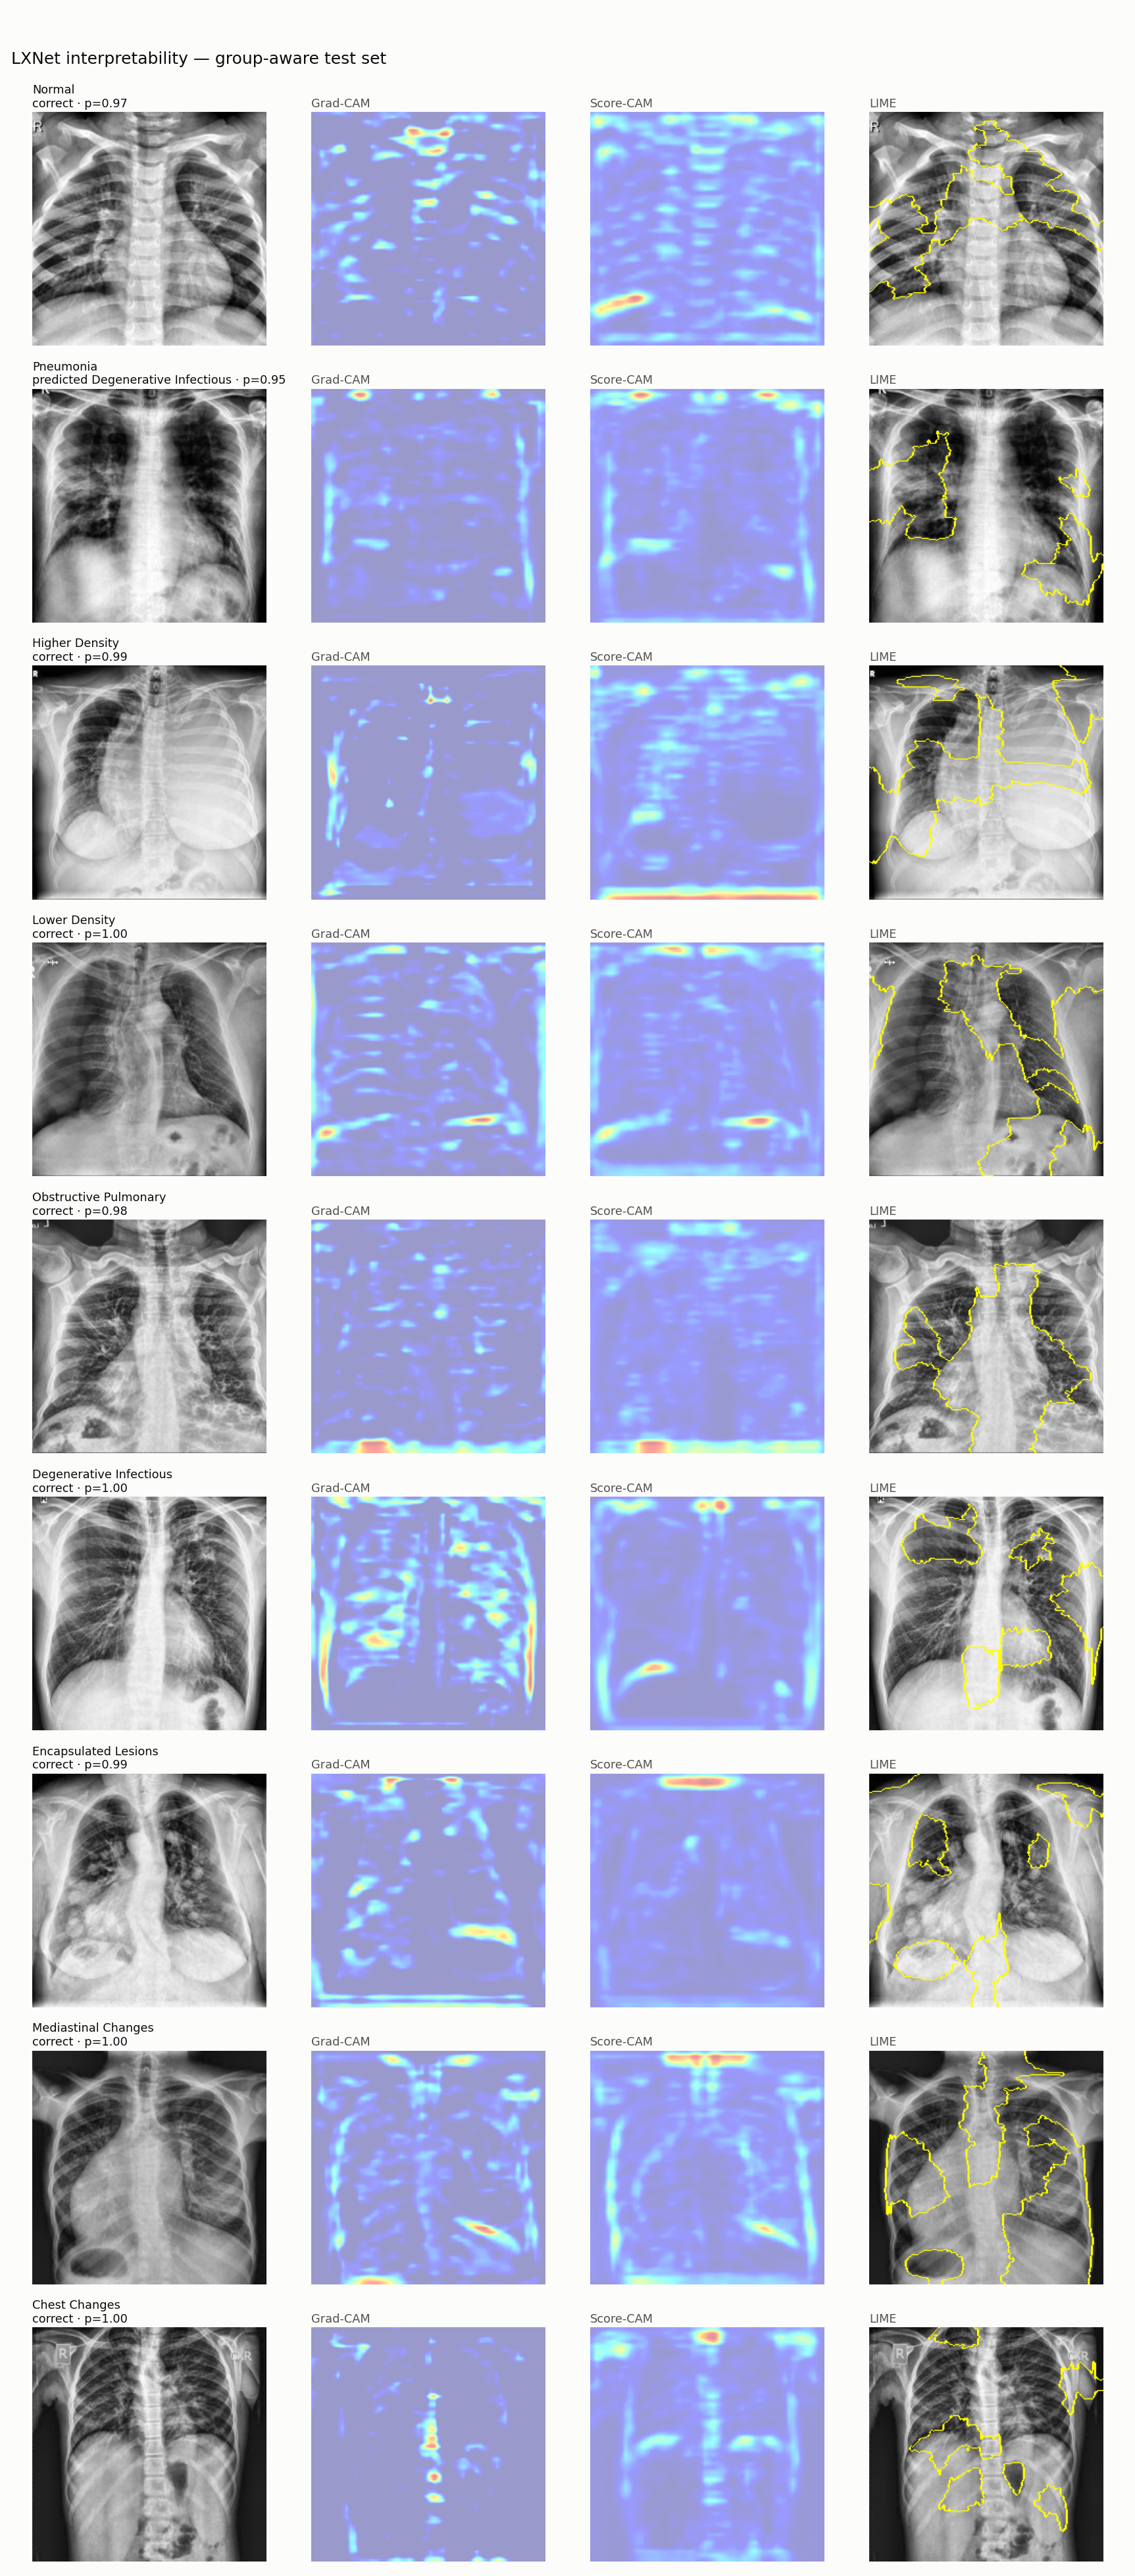
\includegraphics[height=0.86\textheight,keepaspectratio]{fig_xai.png}
\caption{The full interpretability panel, one row per class, group-aware
test set. Column 1: CLAHE'd input with the true class, correctness, and
predicted-class probability. Columns 2--4: Grad-CAM, Score-CAM and LIME for
the predicted class. Row 2 is a genuine failure --- a Pneumonia film
classified as Degenerative Infectious at $p=0.95$ --- shown because a panel
of successes only would not demonstrate anything about failure behaviour.}
\label{fig:xai-panel}
\end{figure}

\section{Reading the Maps Sceptically}

Several attribution maps in \cref{fig:xai-panel} are diffuse, and some place
weight on image borders and edge artefacts rather than lung parenchyma. The
panel is evidence about what the network's final convolutional layer responds
to; it is not a certificate that the network reasons clinically, and a
plausible-looking heatmap centred on a lung is not proof of a correct
mechanism --- a network keying on a scanner-specific artefact that happens to
correlate with lung position would produce an equally plausible-looking map.
This distinction is treated at length in \cref{ch:limitations}.

% ===========================================================================
\chapter{Inference and Deployment}
\label{ch:inference}

\section{The Trust Boundary}

Every module upstream of \code{predict.py} operates on data this system has
already indexed, hashed and audited. \code{predict.py} is where that
assumption ends: its input is a file path handed in by a caller, about which
nothing is known. \code{validate\_image\_path} checks existence, that the
path is a file and not a directory, non-zero size, decodability (via
\code{PIL.Image.verify}, which parses headers without decoding pixel data),
and a minimum dimension of 32\,px --- below which an image carries no
diagnostic content once resized to $224\times224$ and is almost certainly a
thumbnail, an icon, or a failed decode rather than a radiograph.

\begin{lstlisting}[caption={Validation happens before anything expensive
touches the input (\texttt{lxnet/predict.py}).}, label=lst:validate]
class InvalidImageError(ValueError):
    """The input is not a usable image. Distinct from 'the model is
    unsure'."""

def validate_image_path(path: str | Path) -> Path:
    path = Path(path)
    if not path.exists():
        raise FileNotFoundError(f"no such file: {path}")
    ...
    if min(width, height) < MIN_DIMENSION:
        raise InvalidImageError(
            f"image is {width}x{height}; smaller than {MIN_DIMENSION}px "
            f"carries no diagnostic content once resized to "
            f"{IMAGE_SIZE[0]}x{IMAGE_SIZE[1]}"
        )
    return path
\end{lstlisting}

\code{InvalidImageError} is a distinct exception type from
\code{FileNotFoundError} deliberately: "this input cannot be classified" and
"the model classified it with low confidence" are different failure modes,
and a caller (or the CLI) needs to be able to tell them apart rather than
catching a single generic exception and losing that distinction.

\section{Preprocessing Parity}

\code{predict.Classifier.predict} calls the identical
\code{preprocess.load\_image} function that \code{pipeline.build\_cache}
uses to build the training cache (\cref{sec:caching}), not a re-implementation
of it. Preprocessing drifting between training and inference --- a resize
interpolation mode that differs, a CLAHE parameter that differs, a channel
order that differs --- is a classic production failure mode precisely
because it does not raise an exception; it just quietly degrades accuracy in
a way that is easy to miss until someone notices the deployed model
underperforms its evaluated numbers. \texttt{tests/test\_predict.py} pins
this by construction (\cref{ch:testing}).

\section{The \code{Classifier} Interface}

\code{Classifier} loads a checkpoint once at construction (validating that
the checkpoint file exists, with a message pointing at \code{lxnet-train}
if it does not) and exposes \code{predict} (single image, full ranked
distribution) and \code{predict\_many} (batch over file paths, where one bad
file does not abort the rest of the batch --- each failure is caught,
logged, and recorded per-path rather than propagated).

\begin{lstlisting}[caption={A batch of predictions is not aborted by one bad
file (\texttt{lxnet/predict.py}).}, label=lst:predictmany]
def predict_many(self, paths) -> dict[str, list[Prediction] | str]:
    results: dict[str, list[Prediction] | str] = {}
    for p in paths:
        try:
            results[str(p)] = self.predict(p)
        except (FileNotFoundError, InvalidImageError) as exc:
            log.warning("skipping %s: %s", p, exc)
            results[str(p)] = f"error: {exc}"
    return results
\end{lstlisting}

Class name ordering is derived from \code{sorted(CLASS\_LABELS)}, matching
exactly how \code{data.index\_dataset} assigns integer labels by sorted
class-directory name (\cref{ch:dataset}) --- the code comment on this line is
explicit that this must be sorted order, not dictionary insertion order,
because the two coincide today only by construction of the \code{CLASS\_LABELS}
dictionary literal, not by any enforced invariant.

\section{Command-Line Interface}

\code{lxnet-predict} classifies one or more images, printing a ranked
top-$k$ (default 3) probability list per image, or machine-readable JSON with
\code{-{}-json}. A research-use disclaimer is printed to stderr by default
(suppressible with \code{-{}-quiet}) and is deliberately ASCII-only ---
\LXNet{}'s default console encoding on Windows is \texttt{cp1252}, under
which an em dash renders as a replacement character rather than the intended
glyph. The process exit code is non-zero only when \emph{every} input failed,
so a caller can branch on total failure without treating one bad file in a
batch as a fatal condition. Full flag reference: \cref{tab:cli-predict}.

\section{Packaging}

\LXNet{} ships as a standard \code{setuptools}-backed Python package
(\texttt{pyproject.toml}), installable with \code{pip install -e .} and
exposing four console-script entry points
(\cref{tab:cli-predict,tab:cli-train,tab:cli-report,tab:cli-explain}). The
TensorFlow dependency is pinned exactly at \code{2.10.1}: it is the last
TensorFlow release with native Windows GPU support, which is the platform
this system was trained and evaluated on, and \code{2.11+} silently drops to
CPU-only operation on Windows rather than failing to install --- a pin, not a
floor, and a direct consequence of the same GPU-visibility failure mode
discussed in \cref{sec:gpu-guard}.

% ===========================================================================
\chapter{Testing and Continuous Integration}
\label{ch:testing}

\section{Design Philosophy}

The system's test suite is organised around a specific, narrow goal: pin the
failure modes that produce a \emph{plausible wrong number} rather than a
crash. A stack trace is a cheap bug --- it is loud, it blocks the run, and
someone fixes it before results ship. The failure modes this project exists
to prevent (\cref{ch:intro}) are the opposite: they produce a number that
looks like a legitimate accuracy score and is quietly wrong. Every test file
below is written against that threat model.

\begin{table}[h]
\centering
\small
\begin{tabularx}{\linewidth}{@{}l X@{}}
\toprule
\textbf{Test file} & \textbf{Guarantee pinned} \\
\midrule
\code{test\_data.py} & Deduplication, cross-class conflict handling, and
  the ordering constraint between splitting and balancing
  (\cref{sec:balance-order}). \\
\code{test\_grouping.py} & Perceptual near-duplicate detection and
  group-aware splitting --- specifically, that no perceptual group is ever
  cut across a split boundary. \\
\code{test\_preprocess.py} & CLAHE increases local contrast, preserves
  image geometry, and produces network-ready tensors from grayscale, RGB
  and RGBA sources alike. \\
\code{test\_pipeline.py} & Image/label alignment survives the cache
  round-trip, and augmentation never reaches validation or test batches. \\
\code{test\_models.py} & \LXNet{}'s parameter count stays under the
  500{,}000 budget (paper claim: $\approx$0.35\,M); baseline construction
  produces the expected head shape. \\
\code{test\_train\_cli.py} & The GPU guard refuses CPU training by
  default (\cref{sec:gpu-guard}), and cross-validation's early-stopping
  monitor is carved from training rows, not from the scored fold
  (\cref{sec:carve-validation}). \\
\code{test\_evaluate.py} & Macro averaging behaves correctly on imbalanced
  inputs; the Wilcoxon comparison handles the degenerate all-zero-difference
  case (\cref{ch:evaluation}). \\
\code{test\_xai.py} & Grad-CAM and Score-CAM maps have the correct shape,
  are normalised, are class-dependent (a different requested class produces
  a different map), and are not constant --- saliency bugs tend to produce a
  plausible-looking blob rather than an exception. \\
\code{test\_explain.py} & The interpretability panel driver's contract:
  correct row/column construction from a checkpoint and a set of examples. \\
\code{test\_predict.py} & The inference trust boundary rejects invalid
  input before it reaches the model, and inference preprocessing matches
  training preprocessing bit-for-bit (\cref{ch:inference}). \\
\code{test\_report.py} & \texttt{results.json} deterministically produces
  the expected tables and figure set. \\
\bottomrule
\end{tabularx}
\caption{Test files mapped to the specific regression each one exists to
catch, not just the module each one happens to cover.}
\label{tab:test-map}
\end{table}

\section{Continuous Integration}

\Cref{fig:ci} outlines the two-job GitHub Actions workflow
(\texttt{.github/workflows/ci.yml}). The dataset is not checked into the
repository and the slow-marked tests download ImageNet weights, so CI runs
exclusively against synthetic fixtures with \code{pytest -m "not slow"} and
must stay green without either.

\begin{table}[h]
\centering
\small
\begin{tabularx}{\linewidth}{@{}l X@{}}
\toprule
\textbf{Job} & \textbf{Purpose} \\
\midrule
\code{test} & Lint (\code{ruff check}), format check (\code{ruff format
  -{}-check}), and the full non-slow test suite with coverage. \\
\code{guarantees} & Re-runs specifically
  \code{test\_grouping.py}, \code{test\_data.py}, \code{test\_train\_cli.py}
  and \code{test\_predict.py} as their own job, so a leakage or
  monitor-peeking regression fails as its own named check in the pull-request
  status list rather than being buried inside a hundred-line pytest summary. \\
\bottomrule
\end{tabularx}
\caption{CI jobs, \texttt{.github/workflows/ci.yml}. Splitting
\code{guarantees} out of \code{test} is a visibility decision, not a
technical necessity --- both jobs run the same suite on the same commit; the
split exists so a reviewer scanning a checks list sees the evaluation-integrity
guarantees fail by name.}
\label{tab:ci-jobs}
\end{table}

\begin{figure}[htbp]
\centering
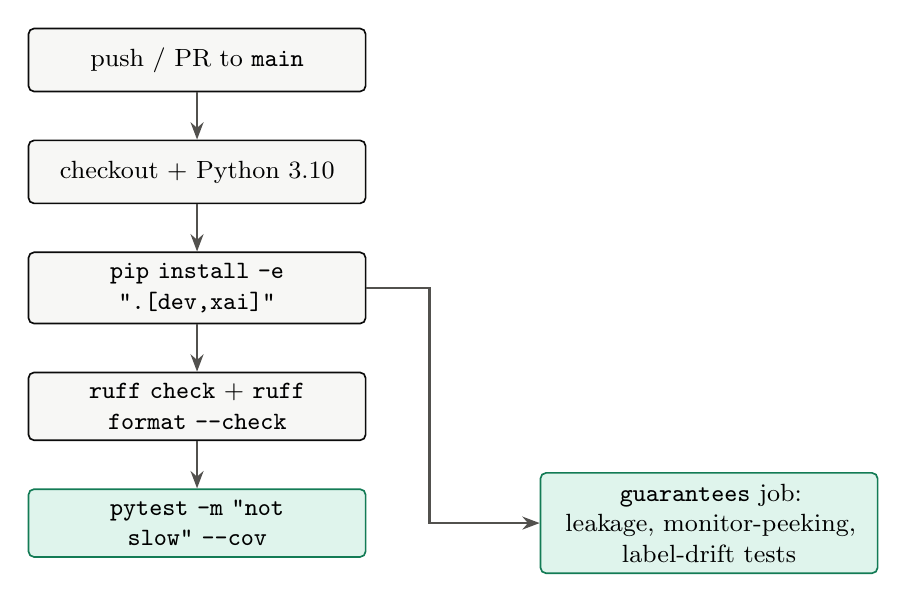
\begin{tikzpicture}[
  node distance=6mm and 10mm,
  every node/.style={font=\small, align=center},
  n/.style={draw=inkblack, rounded corners=2pt, fill=panelbg, minimum height=8mm,
            text width=40mm, inner sep=4pt, line width=0.6pt},
  gate/.style={n, fill=goodgreen!14, draw=goodgreen!70!black},
  arr/.style={-{Stealth[length=2.2mm]}, line width=0.8pt, color=mutedgray},
]
  \node[n] (push) {push / PR to \code{main}};
  \node[n, below=of push] (checkout) {checkout + Python 3.10};
  \node[n, below=of checkout] (install) {\code{pip install -e ".[dev,xai]"}};
  \node[n, below=of install] (lint) {\code{ruff check} + \code{ruff format --check}};
  \node[gate, below=of lint] (test) {\code{pytest -m "not slow" --cov}};
  \node[gate, right=22mm of test] (guarantees) {\code{guarantees} job:\\leakage, monitor-peeking,\\label-drift tests};

  \draw[arr] (push) -- (checkout);
  \draw[arr] (checkout) -- (install);
  \draw[arr] (install) -- (lint);
  \draw[arr] (lint) -- (test);
  \draw[arr] (install.east) -- ++(8mm,0) |- (guarantees.west);
\end{tikzpicture}
\caption{CI pipeline. \code{test} and \code{guarantees} run in parallel from
independent checkouts; both must pass for the workflow to succeed.}
\label{fig:ci}
\end{figure}

% ===========================================================================
\chapter{Engineering Decision Ledger}
\label{ch:decisions}

The preceding chapters justify each decision in place, next to the code it
governs. This chapter collects them in one location, because a decision that
is easy to find is a decision that is easy to revisit correctly rather than
re-litigate from scratch.

\begin{longtable}{@{}p{3.1cm}p{4.6cm}p{6.5cm}@{}}
\toprule
\textbf{Decision} & \textbf{Alternative considered} & \textbf{Why this way} \\
\midrule
\endfirsthead
\toprule
\textbf{Decision} & \textbf{Alternative considered} & \textbf{Why this way} \\
\midrule
\endhead
Exact-match perceptual grouping (\cref{sec:perceptual-grouping}) &
  Fuzzy Hamming-distance matching &
  Measured: any tolerance $\geq 1$ bit chains distinct images into a single
  1{,}680-image group spanning 8 of 9 classes via transitive closure.
  Exact match is the only threshold that does not do this. \\
Split first, balance after (\cref{sec:balance-order}) &
  Balance the whole dataset, then split &
  The paper's ordering places duplicated minority-class images on both
  sides of the split, inflating recall on exactly the classes the technique
  was meant to help. \\
Carve the early-stopping monitor from each fold's training rows
  (\cref{sec:carve-validation}) &
  Monitor \code{val\_loss} on the fold being scored &
  \code{restore\_best\_weights} turns the reported score into a maximum over
  up to 40 epochs if the monitor and the scored fold are the same data. \\
Refuse to train on CPU by default (\cref{sec:gpu-guard}) &
  Fall back to CPU silently &
  TF 2.10 on Windows loses CUDA visibility silently when invoked outside an
  activated Conda environment, turning a 40-minute run into an overnight one
  with no error anywhere in the log. \\
Global average pooling, not \code{Flatten} (\cref{ch:architecture-model}) &
  Flatten $\to$ Dense(256) &
  Flattening the final $28\times28\times128$ map costs 25.7\,M weights on
  that layer alone --- 70$\times$ the entire network's actual budget. \\
CAM attachment on post-activation ReLU, not raw \code{Conv2D}
  (\cref{sec:cam-attachment}) &
  Attach to the raw convolution output &
  The raw output is pre-BatchNorm (arbitrary per-channel scale) and signed;
  Grad-CAM is defined over a non-negative, comparable feature map. \\
Cache preprocessing as grayscale \code{uint8}, not float32 RGB
  (\cref{sec:caching}) &
  Store the fully-prepared model-input tensor &
  12$\times$ smaller on disk (338\,MB vs.\ 4\,GB); channel replication and
  float scaling are cheap enough to do inside the \code{tf.data} graph on
  every batch. \\
Macro-averaged metrics throughout (\cref{ch:evaluation}) &
  Micro (support-weighted) averaging &
  The dataset runs 1{,}340 Normal against 544 Chest Changes; micro averaging
  would let a model that neglects the smallest classes still post a
  flattering headline number. \\
Retain the leaky random-split protocol in the codebase
  (\cref{ch:architecture}) &
  Delete it once the honest protocol was built &
  The leakage measurement in \cref{ch:results} is only meaningful because
  both protocols run on identical images, preprocessing and model code ---
  deleting the leaky path would remove the ability to quantify what it cost. \\
Non-parametric paired significance test (\cref{ch:evaluation}) &
  A parametric paired $t$-test &
  Five cross-validation folds is far too few to justify assuming the
  per-fold score differences are normally distributed. \\
Read image bytes via buffer + \code{cv2.imdecode}, not
  \code{cv2.imread(path)} (\cref{sec:caching}) &
  \code{cv2.imread} directly on the file path &
  \code{cv2.imread} cannot open non-ASCII paths on Windows; the dataset's
  class directories are named in Portuguese. \\
Distinct \code{InvalidImageError} from \code{FileNotFoundError}
  (\cref{ch:inference}) &
  One generic exception type for all input failures &
  ``This input cannot be classified'' and ``the file does not exist'' are
  different failure modes a caller needs to branch on separately. \\
\bottomrule
\caption{Engineering decisions with an alternative that was measured or
seriously considered and rejected, not merely available in principle.}
\label{tab:decision-ledger}
\end{longtable}

% ===========================================================================
\chapter{Limitations and Ethical Considerations}
\label{ch:limitations}

\begin{warningbox}
This is not a medical device and must not be used to make clinical
decisions. Every number in this report was measured on one public dataset of
unknown clinical provenance, and none of it has been validated against a
clinical reference standard.
\end{warningbox}

\section{Intended Use}

\subsection{In Scope}
\begin{itemize}
\item Research on lightweight architectures for radiograph classification.
\item A worked example of near-duplicate–aware evaluation, which is the
  purpose this repository exists to demonstrate.
\item Education: a small model that trains end-to-end on one consumer GPU in
  approximately 40 minutes.
\item A baseline to beat.
\end{itemize}

\subsection{Explicitly Out of Scope}
\begin{itemize}
\item Any clinical use: diagnosis, triage, screening, or second reads.
\item Any use where a missed finding causes harm --- Pneumonia recall is
  73.2\%.
\item Populations, scanners, or acquisition protocols unlike the training
  corpus, which is itself undocumented --- effectively, this excludes
  \emph{any} population with confidence.
\item Paediatric imaging, portable or bedside films, and lateral views. The
  training data's composition on these dimensions is unknown and unverified.
\end{itemize}

\section{Numbered Limitations}

\begin{enumerate}[label=\textbf{L\arabic*.}, leftmargin=2.2em]

\item \textbf{Pneumonia recall is 73.2\%.} This is the single most important
  number in this report. 8\% of pneumonia films are classified \emph{Normal}
  --- a false negative on the most common actionable finding in the dataset.
  Any use that treats a \emph{Normal} output as reassurance is a misuse of
  this system.

\item \textbf{Normal recall is 88.6\%.} The two classes a screening tool
  exists to separate --- Normal and Pneumonia --- are the two classes every
  model tested is worst at (\cref{tab:recall-by-class}). The remaining seven
  classes sit at 94--100\% recall and carry the headline accuracy figure.

\item \textbf{Measured accuracy is dataset-specific and probably
  optimistic.} Seven of nine classes scoring near-100\% recall, uniformly
  across four architecturally unrelated models, is not a realistic
  difficulty profile for chest radiography as a diagnostic task. It more
  plausibly indicates that those classes are separable by acquisition
  artefacts --- scanner make, exposure setting, framing, or collection
  source --- than that any of the four models has learned the underlying
  pathology. This has not been tested directly and should be assumed true
  until disproven.

\item \textbf{No external validation.} One dataset, one split protocol, and
  --- probably, though provenance is undocumented --- one institution's worth
  of imaging. Nothing measured in this report predicts behaviour on a
  different hospital's films, a different scanner vendor, or a different
  patient population.

\item \textbf{Class definitions are coarse and non-standard.} ``Higher
  Density'' bundles effusion, consolidation, hydrothorax and empyema ---
  clinically distinct entities with different causes and different
  management pathways. The nine-class label set used throughout this report
  is not a validated clinical taxonomy.

\item \textbf{The interpretability maps are weak evidence, not proof.}
  Several Grad-CAM and Score-CAM maps in \cref{fig:xai-panel} are diffuse or
  weight image borders rather than lung tissue. They demonstrate what the
  final convolutional layer responds to; they do not demonstrate clinical
  reasoning (\cref{ch:xai}).

\item \textbf{No calibration.} Softmax outputs are not calibrated
  probabilities. A reported confidence of 0.95 is not a measured 95\% chance
  of correctness --- this system has not been assessed for expected
  calibration error, reliability diagrams, or behaviour under distribution
  shift.

\item \textbf{No out-of-distribution detection.} Given a hand radiograph, an
  abdominal film, or an arbitrary photograph, the system returns a confident
  nine-class probability distribution over chest pathologies. It has no
  mechanism to recognise ``this is not a chest X-ray.''

\end{enumerate}

\section{Training Data Provenance}

Known and handled: 85 byte-identical duplicate files (removed before
splitting); one image filed under two contradictory classes (both copies
dropped, \cref{sec:exact-dedup}); 30\% visual redundancy across the
byte-unique corpus, addressed by group-aware splitting
(\cref{sec:group-aware-split}); 40 distinct resolutions and mixed
grayscale/RGB/RGBA colour modes, normalised in preprocessing
(\cref{ch:preprocessing}).

Unknown and unverifiable from the data as distributed: patient identities;
whether a single patient contributes multiple films; scanner make, model, and
acquisition parameters; geographic and demographic composition; label
provenance, and whether labels were subject to any clinical adjudication.
\textbf{No demographic breakdown of model performance is possible} on this
dataset, and fairness across sex, age, or ethnicity is therefore untested ---
a serious and unresolved gap for any system that touches medical imaging.

\section{Ethical Considerations}

Deploying an automated reader into any diagnostic pathway shifts risk onto
patients who did not consent to it and, in most workflows, cannot see it
happening. The failure mode that matters clinically is not average accuracy
but the missed finding: at 73\% pneumonia recall, a system trusted as a
first-pass filter would send roughly one in four pneumonia patients away with
a falsely reassuring result.

Automation bias compounds this risk independently of raw accuracy: a
confident label presented to a time-pressured reader measurably shifts their
judgement even when the label is wrong, and a plausible-looking
interpretability overlay (\cref{ch:xai}) makes an incorrect prediction
\emph{more} persuasive to a human reviewer, not less.

Absent any demographic metadata, this system cannot be audited for
differential performance across patient subgroups. A model that measures 93\%
accurate in aggregate can be substantially worse for an under-represented
subgroup, and nothing in the current dataset or evaluation protocol would
reveal that gap if it exists.

% ===========================================================================
\chapter{Reproducibility}
\label{ch:reproducibility}

\section{Environment}

\begin{table}[h]
\centering
\small
\begin{tabular}{@{}ll@{}}
\toprule
\textbf{Component} & \textbf{Pinned version} \\
\midrule
Python & 3.10 (\code{>=3.10,<3.11}) \\
TensorFlow & 2.10.1 exactly (\cref{ch:inference}) \\
NumPy & \code{>=1.23,<2.0} \\
OpenCV (\code{opencv-python}) & \code{>=4.7} \\
Pillow & \code{>=9.0} \\
scikit-learn & \code{>=1.2} \\
SciPy & \code{>=1.9} \\
matplotlib & \code{>=3.6} \\
pandas & \code{>=1.5} \\
Optional (\code{xai} extra) & \code{lime>=0.2.0.1}, \code{scikit-image>=0.19} \\
\bottomrule
\end{tabular}
\caption{Pinned dependency versions, \texttt{pyproject.toml}.}
\label{tab:deps}
\end{table}

\section{Reproducing the Reported Numbers}

\begin{lstlisting}[language=bash, caption={The exact commands that produced
every table and figure in \cref{ch:results}.}, label=lst:repro]
pip install -e ".[dev,xai]"

python -m lxnet.train --out-dir runs/grouped \
    --split-mode grouped --cv-models LXNet

python -m lxnet.train --out-dir runs/random \
    --split-mode random --models LXNet --cv-models LXNet

python -m lxnet.report
\end{lstlisting}

To populate the significance test left unrun in \cref{sec:significance},
cross-validate a second model against the same folds, for example:

\begin{lstlisting}[language=bash]
python -m lxnet.train --out-dir runs/grouped \
    --split-mode grouped --models ResNet50V2 --cv-models ResNet50V2
\end{lstlisting}

\section{Reproducibility Record}
\label{sec:repro-record}

\begin{table}[h]
\centering
\small
\begin{tabular}{@{}lll@{}}
\toprule
 & \textbf{Group-aware arm} & \textbf{Random arm} \\
\midrule
Split mode & \code{grouped} & \code{random} \\
Train / val / test & 4{,}660 / 1{,}000 / 997 & 4{,}660 / 999 / 998 \\
Seed & 42 & 42 \\
Max epochs & 40, patience 8 & 40, patience 8 \\
Batch size & 32 & 32 \\
\bottomrule
\end{tabular}
\caption{Reproducibility record. Both arms consume the same cached CLAHE'd
tensor (\cref{sec:caching}), so preprocessing is bit-for-bit identical
between them --- the split function is the only variable that differs.}
\label{tab:repro-record}
\end{table}

Every figure in \cref{ch:results} is generated programmatically by
\code{python -m lxnet.report} directly from \texttt{results.json}; none is
drawn or edited by hand, and re-running the report step against the same
\texttt{results.json} is idempotent.

\section{Hardware}

Measured training times in \cref{tab:training-cost} are single-GPU wall
clock on the machine this replication was run on; absolute times will vary
by GPU model and driver, but relative ordering (backbones finish in roughly a
third the time of \LXNet{}, despite $50$--$70\times$ more parameters, because
their weights are frozen) should hold generally, since it follows from the
computation performed rather than from the specific hardware.

% ===========================================================================
\chapter{Conclusion and Future Work}
\label{ch:conclusion}

\section{Summary}

This report documented a system built around one falsifiable measurement:
that a naive evaluation split on this dataset overstates accuracy by 2.5
percentage points on the hold-out set and by a wider, less stable margin
under cross-validation, because 30\% of the corpus is redundant and a random
split does not respect that redundancy. Removing the leak required changes
at every layer --- exact and perceptual deduplication, group-aware splitting
and folding, balancing after rather than before splitting, and an
early-stopping regime that cannot peek at the fold it reports --- and each of
those changes is now pinned by an automated test so it cannot silently
regress (\cref{ch:testing}).

The result the system was built to test survives the correction, in a
qualified form: \LXNet{} does not match the largest backbone's accuracy
(92.9\% versus ResNet50V2's 98.5\%), but it reaches that accuracy at
$1/67$\textsuperscript{th} the parameter count, a trade that is legitimate
engineering rather than an artefact of the evaluation protocol.

\section{Future Work}

\begin{itemize}
\item \textbf{Populate the significance test} (\cref{sec:significance}) by
  cross-validating at least one backbone alongside \LXNet{}, so the
  parameter-efficiency claim can be stated with a $p$-value rather than a
  single hold-out comparison.
\item \textbf{Test the acquisition-artefact hypothesis} raised in L3
  (\cref{ch:limitations}): if the seven near-100\%-recall classes are
  separable by scanner or source metadata rather than pathology, a model
  trained on metadata alone should approach the same accuracy on those
  classes --- a direct, falsifiable test of the concern rather than a
  standing caveat.
\item \textbf{Carve the cross-validation monitor by perceptual group}
  (\cref{sec:carve-validation}), closing the one documented piece of
  engineering debt in the training path, if the stopping epoch is ever
  observed to be systematically late.
\item \textbf{Calibrate the output probabilities} (L7) and add
  out-of-distribution rejection (L8) before this system's output could be
  responsibly surfaced to any downstream consumer, clinical or not.
\item \textbf{External validation} on a second, independently-sourced chest
  radiograph dataset is the direct test of L4 and would be the single most
  informative next experiment this report does not contain.
\end{itemize}

% ===========================================================================
\appendix

\chapter{Command-Line Interface Reference}
\label{ap:cli}

\section{\code{lxnet-train}}

\begin{table}[h]
\centering
\small
\begin{tabularx}{\linewidth}{@{}lll X@{}}
\toprule
\textbf{Flag} & \textbf{Type} & \textbf{Default} & \textbf{Meaning} \\
\midrule
\code{-{}-data-root} & path & \code{dataset} & Dataset root directory. \\
\code{-{}-out-dir} & path & \code{runs/latest} & Results, checkpoints, and
  preprocessing cache. \\
\code{-{}-models} & list & all four & Subset of models to train. \\
\code{-{}-epochs} & int & 40 & Maximum epochs (early stopping, patience 8). \\
\code{-{}-batch-size} & int & 32 & Training batch size. \\
\code{-{}-folds} & int & 5 & Cross-validation fold count. \\
\code{-{}-seed} & int & 42 & Global random seed. \\
\code{-{}-skip-cv} & flag & off & Hold-out evaluation only, no
  cross-validation. \\
\code{-{}-allow-cpu} & flag & off & Permit training without a visible GPU
  (\cref{sec:gpu-guard}). \\
\code{-{}-limit} & int & --- & Subsample to $N$ images, for smoke testing. \\
\code{-{}-split-mode} & choice & \code{grouped} & \code{grouped} (leak-free)
  or \code{random} (leaky protocol, for comparison). \\
\code{-{}-cv-models} & list & value of \code{-{}-models} & Subset of models
  to cross-validate; the heavy backbones are usually hold-out only for time
  reasons. \\
\bottomrule
\end{tabularx}
\caption{\texttt{lxnet-train} / \texttt{python -m lxnet.train} flags.}
\label{tab:cli-train}
\end{table}

\section{\code{lxnet-predict}}

\begin{table}[h]
\centering
\small
\begin{tabularx}{\linewidth}{@{}lll X@{}}
\toprule
\textbf{Flag} & \textbf{Type} & \textbf{Default} & \textbf{Meaning} \\
\midrule
\code{images} & path(s) & required & One or more image files to classify. \\
\code{-{}-checkpoint} & path & \code{runs/grouped/checkpoints/}\linebreak
  \code{LXNet\_holdout.weights.h5} & Trained weights file. \\
\code{-{}-model} & str & \code{LXNet} & Architecture matching the checkpoint. \\
\code{-{}-top-k} & int & 3 & Classes to display (0 = all). \\
\code{-{}-json} & flag & off & Machine-readable output. \\
\code{-{}-quiet} & flag & off & Suppress the research-use disclaimer. \\
\bottomrule
\end{tabularx}
\caption{\texttt{lxnet-predict} flags.}
\label{tab:cli-predict}
\end{table}

\section{\code{lxnet-report}}

\begin{table}[h]
\centering
\small
\begin{tabularx}{\linewidth}{@{}lll X@{}}
\toprule
\textbf{Flag} & \textbf{Type} & \textbf{Default} & \textbf{Meaning} \\
\midrule
\code{-{}-grouped} & path & \code{runs/grouped/results.json} & Group-aware
  arm results. \\
\code{-{}-random} & path & \code{runs/random/results.json} & Random-split
  arm results (optional; leakage arm reads as pending if absent). \\
\code{-{}-out-dir} & path & \code{docs} & Output directory for figures and
  \texttt{RESULTS.md}. \\
\code{-{}-data-root} & path & \code{dataset} & Needed to recompute the
  leakage fraction reported in \cref{ch:results}. \\
\bottomrule
\end{tabularx}
\caption{\texttt{lxnet-report} flags.}
\label{tab:cli-report}
\end{table}

\section{\code{lxnet-explain}}

\begin{table}[h]
\centering
\small
\begin{tabularx}{\linewidth}{@{}lll X@{}}
\toprule
\textbf{Flag} & \textbf{Type} & \textbf{Default} & \textbf{Meaning} \\
\midrule
\code{-{}-run-dir} & path & \code{runs/grouped} & Directory holding the
  preprocessing cache and checkpoints. \\
\code{-{}-model} & str & \code{LXNet} & Architecture to load and explain. \\
\code{-{}-data-root} & path & \code{dataset} & Dataset root, to re-derive
  the test split. \\
\code{-{}-out} & path & \code{docs/fig\_xai.png} & Output panel image
  (\cref{fig:xai-panel}). \\
\code{-{}-split-mode} & choice & \code{grouped} & Must match the checkpoint's
  training split mode. \\
\code{-{}-seed} & int & 42 & Reproduces the same per-class example choice. \\
\code{-{}-lime-samples} & int & 400 & LIME perturbation sample count
  (\cref{ch:xai}); higher is slower and more stable. \\
\bottomrule
\end{tabularx}
\caption{\texttt{lxnet-explain} flags.}
\label{tab:cli-explain}
\end{table}

% ===========================================================================
\chapter{Repository Layout}
\label{ap:layout}

\begin{lstlisting}[language=bash, basicstyle=\ttfamily\small, frame=single,
  rulecolor=\color{rulegray}, backgroundcolor=\color{panelbg}]
lxnet/
  data.py        indexing, dedup, perceptual grouping, splits, folds
  preprocess.py  CLAHE, image loading
  pipeline.py    cached tf.data input pipeline
  models.py      LXNet + DenseNet201 / ResNet50V2 / InceptionV3
  train.py       hold-out and k-fold orchestration
  predict.py     inference: validation, preprocessing, ranked probabilities
  evaluate.py    metrics, fold summaries, Wilcoxon signed-rank
  xai.py         Grad-CAM, Score-CAM, LIME, overlays
  explain.py     per-class interpretability panel
  report.py      themed figures and docs/RESULTS.md
docs/            results, model card, figures, this report
tests/           the evaluation guarantees are pinned here
runs/            per-experiment checkpoints, caches and results.json
.github/         CI workflow
\end{lstlisting}

% ===========================================================================
\begin{thebibliography}{9}

\bibitem{humayan2026}
Humayan, A. et al.
\textit{A Lightweight CNN for Lung Disease Classification from Chest X-ray
with XAI-based Interpretability.}
PLOS One, 2026.

\bibitem{selvaraju2017}
Selvaraju, R. R., Cogswell, M., Das, A., Vedantam, R., Parikh, D., Batra, D.
\textit{Grad-CAM: Visual Explanations from Deep Networks via Gradient-based
Localization.}
IEEE International Conference on Computer Vision (ICCV), 2017.

\bibitem{wang2020}
Wang, H., Wang, Z., Du, M., Yang, F., Zhang, Z., Ding, S., Mardziel, P., Hu, X.
\textit{Score-CAM: Score-Weighted Visual Explanations for Convolutional
Neural Networks.}
IEEE/CVF Conference on Computer Vision and Pattern Recognition Workshops
(CVPRW), 2020.

\bibitem{ribeiro2016}
Ribeiro, M. T., Singh, S., Guestrin, C.
\textit{``Why Should I Trust You?'': Explaining the Predictions of Any
Classifier.}
ACM SIGKDD International Conference on Knowledge Discovery and Data Mining
(KDD), 2016.

\bibitem{pedregosa2011}
Pedregosa, F. et al.
\textit{Scikit-learn: Machine Learning in Python.}
Journal of Machine Learning Research, 12, 2011.

\bibitem{wilcoxon1945}
Wilcoxon, F.
\textit{Individual Comparisons by Ranking Methods.}
Biometrics Bulletin, 1(6), 1945.

\bibitem{kaggle-dataset}
fernando2rad.
\textit{X-Ray Lung Diseases Images (9 classes).}
Kaggle dataset. \url{https://www.kaggle.com/datasets/fernando2rad/x-ray-lung-diseases-images-9-classes}

\end{thebibliography}

\end{document}





